%% Modified from the original thesisdown template.tex
%%
%% Preamble
%%
\documentclass[12pt]{article}
% Packages are extensions to the basic LaTeX functions. Whatever you
% want to typeset, there is probably a package out there for it.
% Chemistry (chemtex), screenplays, you name it.
% Check out CTAN to see: https://www.ctan.org/
\usepackage{amsmath}
\usepackage{fixltx2e}
\usepackage{graphicx}
\usepackage{longtable}
\usepackage{float}
\usepackage{wrapfig}
\usepackage{soul}
\usepackage{textcomp}
\usepackage{marvosym}
\usepackage{wasysym}
\usepackage{latexsym}
\usepackage{amssymb}
\usepackage{amstext}
\usepackage{amsthm}
\usepackage{chemarr} %% Useful for one reaction arrow, useless if you're not a chem major
\usepackage{booktabs}
\usepackage[hyphens]{url}
\usepackage{hyperref}
\usepackage{lmodern}
\usepackage{float}
\floatplacement{figure}{H}
\usepackage{calc}
\usepackage{rotating}
\usepackage{algorithm}
\usepackage{algpseudocode}

% Loads the YSU Style Package (YSU.sty)
\usepackage{YSU} 

% For pandoc to work
\providecommand{\tightlist}{%
  \setlength{\itemsep}{0pt}\setlength{\parskip}{0pt}}
\providecommand{\pandocbounded}[1]{#1}
% needed for proper highlighting
\usepackage{color}
\usepackage{fancyvrb}
\newcommand{\VerbBar}{|}
\newcommand{\VERB}{\Verb[commandchars=\\\{\}]}
\DefineVerbatimEnvironment{Highlighting}{Verbatim}{commandchars=\\\{\}}
% Add ',fontsize=\small' for more characters per line
\usepackage{framed}
\definecolor{shadecolor}{RGB}{248,248,248}
\newenvironment{Shaded}{\begin{snugshade}}{\end{snugshade}}
\newcommand{\AlertTok}[1]{\textcolor[rgb]{0.94,0.16,0.16}{#1}}
\newcommand{\AnnotationTok}[1]{\textcolor[rgb]{0.56,0.35,0.01}{\textbf{\textit{#1}}}}
\newcommand{\AttributeTok}[1]{\textcolor[rgb]{0.13,0.29,0.53}{#1}}
\newcommand{\BaseNTok}[1]{\textcolor[rgb]{0.00,0.00,0.81}{#1}}
\newcommand{\BuiltInTok}[1]{#1}
\newcommand{\CharTok}[1]{\textcolor[rgb]{0.31,0.60,0.02}{#1}}
\newcommand{\CommentTok}[1]{\textcolor[rgb]{0.56,0.35,0.01}{\textit{#1}}}
\newcommand{\CommentVarTok}[1]{\textcolor[rgb]{0.56,0.35,0.01}{\textbf{\textit{#1}}}}
\newcommand{\ConstantTok}[1]{\textcolor[rgb]{0.56,0.35,0.01}{#1}}
\newcommand{\ControlFlowTok}[1]{\textcolor[rgb]{0.13,0.29,0.53}{\textbf{#1}}}
\newcommand{\DataTypeTok}[1]{\textcolor[rgb]{0.13,0.29,0.53}{#1}}
\newcommand{\DecValTok}[1]{\textcolor[rgb]{0.00,0.00,0.81}{#1}}
\newcommand{\DocumentationTok}[1]{\textcolor[rgb]{0.56,0.35,0.01}{\textbf{\textit{#1}}}}
\newcommand{\ErrorTok}[1]{\textcolor[rgb]{0.64,0.00,0.00}{\textbf{#1}}}
\newcommand{\ExtensionTok}[1]{#1}
\newcommand{\FloatTok}[1]{\textcolor[rgb]{0.00,0.00,0.81}{#1}}
\newcommand{\FunctionTok}[1]{\textcolor[rgb]{0.13,0.29,0.53}{\textbf{#1}}}
\newcommand{\ImportTok}[1]{#1}
\newcommand{\InformationTok}[1]{\textcolor[rgb]{0.56,0.35,0.01}{\textbf{\textit{#1}}}}
\newcommand{\KeywordTok}[1]{\textcolor[rgb]{0.13,0.29,0.53}{\textbf{#1}}}
\newcommand{\NormalTok}[1]{#1}
\newcommand{\OperatorTok}[1]{\textcolor[rgb]{0.81,0.36,0.00}{\textbf{#1}}}
\newcommand{\OtherTok}[1]{\textcolor[rgb]{0.56,0.35,0.01}{#1}}
\newcommand{\PreprocessorTok}[1]{\textcolor[rgb]{0.56,0.35,0.01}{\textit{#1}}}
\newcommand{\RegionMarkerTok}[1]{#1}
\newcommand{\SpecialCharTok}[1]{\textcolor[rgb]{0.81,0.36,0.00}{\textbf{#1}}}
\newcommand{\SpecialStringTok}[1]{\textcolor[rgb]{0.31,0.60,0.02}{#1}}
\newcommand{\StringTok}[1]{\textcolor[rgb]{0.31,0.60,0.02}{#1}}
\newcommand{\VariableTok}[1]{\textcolor[rgb]{0.00,0.00,0.00}{#1}}
\newcommand{\VerbatimStringTok}[1]{\textcolor[rgb]{0.31,0.60,0.02}{#1}}
\newcommand{\WarningTok}[1]{\textcolor[rgb]{0.56,0.35,0.01}{\textbf{\textit{#1}}}}

% From {rticles}

%%% Thesis-specific information
\title{Using Machine Learning to Optimize The Board Game Can't Stop}
\author{J. Cameron Carter}
% NOTE the change to the \date command.  This is important for the copyright page
\date{May}{2026} 
\YSUdegree{Bachelor of Science}{Mathematics/Data Science}
\committee{Dr.~Christopher Mecklin}{Dr.~Md. Mahadi Hasan}{Dr.~Manoj Pathak}

\begin{document}

%%% Frontmatter
\createtitlepage
\createsignaturepage

%%% Copyright page (optional)
%%% YSU Grad College guidelines state to delete this page if copyright
%%% not registered with copyright.gov
\createcopyrightpage

%%% Acknowledgements (optional)
\begin{aknowledgements}
\normalsize
% This is the text of the Acknowledgements

\bigskip

\indent I would like to thank the entire Murray State Department of Mathematics and Statistics, 
my advisor Dr. Mecklin, and my supportive friends and family. A very special thank you to my mom, 
who is the backbone of this project's grammar and spelling. 
This project would not have been possible without all of their wonderful support 
and encouragement. 
\end{aknowledgements}

%%% Abstract is required.  Double-spaced, maximum one (1) page
\begin{abstract}
\normalsize
% This is the text of the Abstract

\bigskip

\noindent Can’t Stop is a jeopardy dice game invented by Sid Jackson and first published in 1980. It has players rolling four dice to make pairs that advance markers up a board, with the first player to complete three columns winning the game. 
One of the most important decisions each turn is deciding whether to stop rolling the dice to keep your progress, or risk failing the next roll and losing your progress. 
Different strategies have been developed on when is the optimal time to stop, using a variety of statistical and mathematical approaches. 
However, one approach that has not seen significant development is neural networks, a machine learning method. 
Through experimentation and computer simulations, 
the goal is to see if using the reinforcement learning algorithm Deep Q-Learning (a type of neural network) will produce a better strategy for when to stop rolling than existing strategies, 
such as Rule of 28 (Keller 1986) or Generalized Heuristic (Glenn and Aloi 2009).

\end{abstract}

%%% Table of contents
\tableofcontents 

%%% List of Tables (optional)
\listoftables

%%% List of Figures (optional)
\listoffigures

%%%%% Main body of Thesis
\begin{thesis}

\newpage

\section{Introduction}\label{intro}

\subsection{Can't Stop Description}\label{cant-stop-description}

Can't Stop is a board game developed by Sid Sackson and published by Parker Brothers in 1980.
It is a two to four player jeopardy dice game where each player tries to get to the top of three columns first.
We define a jeopardy dice game as a game that uses one or more dice as a random device, where the main decision is whether or not to jeopardize previous gains by rolling dice for possible greater gains with a risk of losing all gains from that turn.

In Can't Stop, during a player's turn they roll 4 six-sided dice, which will allow the player to either make progress (greater gains) towards the top of a column or reset their progress (jeopardize previous gains) and end the turn.

Other games in the jeopardy dice game genre include Pig, Cosmic Wimpout, Twenty-One, and Macao.

\begin{figure}

{\centering 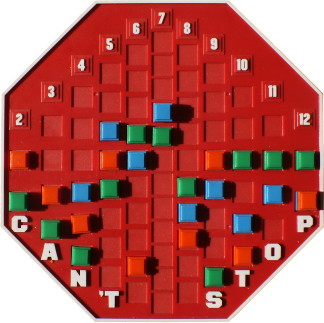
\includegraphics[width=0.4\linewidth,alt={A game of Can't Stop in Progress}]{figure/CantStopsm} 

}

\caption{Sample Can't Stop game in progress}\label{fig:gameboard}
\end{figure}

\footnote{Figure \ref{fig:gameboard} Retrieved from \url{https://en.wikipedia.org/wiki/Can\%27t_Stop_(board_game)}}

Informally, we define a game as competitive rule-based play involving multiple players.
The players take turns making progress towards a goal, and the first player to reach this goal is deemed the winner.
A mathematical definition of a game is the specification of a set of players, rules for playing the game, and an assignment of payoffs or utilities to all possible endings resulting from the various actions of the players.
Rules specify the order and consequence of moves for the various players, how the game ends, and who gets what under various endings (Packel 2006).
We can further define a player and payoff as someone who makes choices and receives payoffs, and a positive or negative number assigned to each possible game end respectively (Rapoport 1966).
While there are different types of games based on the overall payoff, we will only consider zero-sum games, a game where the players' payoffs sum to zero. Can't Stop is a zero-sum game.

A zero-sum game is a game of competitive interactions where one player's gain is another player's loss.
These types of games can be solved, which means we can determine the outcome or possible outcomes of each game, given certain assumptions about the players.
These solutions develop into a strategy, where the answer to a player's choices are specified in advance.
The optimal play, also referred to as a saddle point or minimax, is the move that maximizes your payoff while minimizing your opponent's payoff based on the opponent's move choice.
For each move you can make, you assume your opponent picks your worst-case scenario loss.
From all the possible worst cases, pick the move that with the smallest loss.
This process is minimizing your maximum losses.
The other player will do the opposite, trying to maximize their minimum gains.
The move choices of each player will result in optimal play.
Assuming both players will act rationally and an optimal play exists, then both players will always have to pick the same move, since that move's payoff is the best they can do knowing the other will act rationally.
A dominant strategy is mathematically unexploitable by other players, ensuring positive payoff regardless of your opponent's actions.
Regardless of the opponent's move choice, you will always be maximizing your gains.
Exploitable play uses opponents' mistakes and strategies to maximize your own payoff, by targeting an identified weakness.

As an example, here is how these different strategies would look like in the game Rock-Paper-Scissors.
The optimal play is to pick one of the three options randomly.
Since you assume your opponent is playing rationally, the random choice maximizes your winning chance without giving your opponent an advantage, minimizing their winning chance.
A dominant strategy would be if one player could use a hypothetical fourth move, such as ``dynamite'', that always wins.
This move would be a dominant strategy for that player.
The exploitable play would be a scenario where you notice the opponent always picks rock on the second round, so you exploit this behavior by always picking paper on the second round.
However, while adopting an exploitive strategy can increase your gains, it exposes you to being re-exploited by your opponent.
In the Rock-Paper-Scissors situation, if you start always picking paper, a clever opponent will start picking scissors.

Another example of exploitive play is in the card game poker. In poker players often can take advantage of their opponent's mistakes, like never bluffing or bluffing too often. This would not be an optimal play because the player's strategy is not assuming the opponent is making their best decisions. Since the opponent is not making optimal decisions the player can exploit their opponent.

\subsection{Game Materials}\label{game-materials}

The board consists of 11 columns, numbered 2 through 12, with lengths 3, 5, 7, 9, 11, 13, 11, 9, 7, 5, and 3 respectively.
The game uses 4 six-sided dice, four colored sets of 11 markers, and three neutral-colored markers (runners).

\subsection{Rules}\label{rules}

On a player's turn, they roll all 4 six-sided dice at once.
They form two pairs of numbers with the dice that they have rolled.
The sums of these pairs determine the column(s) in which the player must introduce a runner.
You may have only a total of 3 runners active in any given turn.

The player rerolls all 4 dice and again forms two dice pairs.
After doing so, they again introduce or move one or two runners.

Turns continue like this until the player stops voluntarily or is forced to stop because they cannot introduce or move a runner.

If a player stops voluntarily, they replace each of their runners with one of their markers on the game board.
If during a later turn, the player introduces a runner in a column that already has a marker, they place the runner on the square above the one occupied by their marker.

If a player is forced to stop, they remove the runners from the board, losing all progress achieved that turn, and their turn ends. This is referred to as a bust, or busting.

If a player's runner reaches the top of the column, and then they choose to stop, the player wins that column.
The player to win 3 columns first wins the game.

As an example, consider this scenario:

At the start of a player's turn, they roll the 4 dice and get 2,3,4,5.
Then the possible pairs are (2+3,4+5), (2+4,3+5), or (2+5,3+4), giving the player either (5,9), (6,8), or (7,7).
If the player chooses the first pair, they place a runner on the bottom square of the 6 column and another runner at one the bottom square of the 9 column.
If the player chooses the second pair, they place a runner on the bottom square of the 6 column and another runner on the bottom square of the 8 column.
If the player chooses the third pair, they place a runner on the bottom square of the 7 column and then move it one square upwards.
Each roll will result in at most three distinct pairs.
A roll can return less than three possible pairs, such as 1,1,5,6 which gives (2,11) or (7,6), 3,3,3,5 which gives (6,8), or 4,4,4,4 which gives (8).

\newpage

\section{Literature Review}\label{lit-rev}

Research on finding optimal strategies and solving Can't Stop has been ongoing since the game's release in 1980.
A main focus is developing a heuristic strategy or ``rule of thumb'', defined as a strategy that is easy and quick to execute for any player while gaining a meaningful advantage over other players.
The earliest heuristic strategy is the Rule of 28 (Keller 1986).
This strategy creates an easy-to-remember system of point scoring based on column and move choices, where the player stops upon reaching a score threshold of 28.
The points for each column are based on the probability of getting that column in a roll, with more likely numbers being assigned less points, and unlikely numbers assigned high points.
The Rule of 28 (Ro28) serves as a useful benchmark for developing other strategies.

A common approach to finding strategies is using computer simulations to approximate or solve a game.
Complicated games like Can't Stop are difficult to solve due to the computation time, so breaking the game down into simple, solitaire versions or ``toy'' games, which are solvable can provide useful insight into the full game.
The Retrograde Approximation Algorithms have solved simple versions of one-player games, up to 5-sided dice with the shortest column of length 2.
2-player games were solved up to 4-sided dice with a shortest column of 1 (Fang, Glenn, \& Kruskal 2008).
These algorithms combine Newton's method and retrograde analysis to solve the game by modeling it as a finite, cyclic graph which can be used to show the existence of unique optimal solutions.
The algorithms are iterated over the graph representations until the algorithm converges to a value after enough time.
From the value they get the game theoretic optimal play.
From these solutions, patterns can be found to approximate optimal strategies for the full game.

The Rule of 28 heuristic was generalized, so it can be used for the toy games (Glenn \& Aloi 2009).
However, with the generalized heuristic there are many new factors to consider adding for the scoring, such as difficulty values for each column, the weight of individual moves, difficulty scores for different column combinations, and the current positions of markers.
Glenn \& Aloi used a genetic algorithm to optimize these factors' scoring values, involving encoding different parts of the game to be run for over 250,000 simulated games.
They found their genetic algorithm when ran against the pure Rule of 28 in toy versions, showing an improvement over the Rule of 28.
From this improved toy Can't Stop strategy, we can see that there is possible improvement over the Rule of 28, which could translate into the full game.

Another similar game to Can't Stop is backgammon, a very popular gambling dice game with a body of research on developing different optimized strategies and computer algorithms.
In backgammon, two players are racing their pieces to their home spot.
If a piece is alone at a stage, the opponent can ``blot'' it, sending back to the start, resetting your progress.
Because of the dice rolling, race to finish first, and possibility to lose progress, backgammon strategies and their development process can provide insight into researching Can't Stop.
One backgammon method with successful application to Can't Stop is the rollout method, which resulted in a Can't Stop program that wins most games (Canakci, Serrano, Roy, \& Kruskal 2016).
A rollout is a Monte Carlo evaluation of a position in which the computer plays a position to completion many times (typically thousands of trials), using different random dice sequences in each trial (Tesauro 2002).
The rollout method determines the best move by playing the game thousands of times against itself using each option and then picks the option with the best win rate.
While this approach wins, it wins via complex computations which are difficult to fully integrate into a heuristic strategy that can be implemented by a human.
However, we can analyze the computer play to gain insight into new approaches.
The other approach they used was neural networks, a machine learning method.
They chose to use a self-teaching network similar to the backgammon network TDGammon.
Due to the long training period required to get desirable results, this method was ultimately abandoned despite showing some promise.
If we train a computer to play Can't Stop, then we can try to gain insight into new approaches to a heuristic strategy.

Machine learning is the study of artificial intelligence focused on the development of statistical algorithms that learn from data to make accurate inferences about new unseen data.
Neural networks are a machine learning model that takes inputs, passes it through neurons to transform the inputs, and then an activation function outputs a prediction.
Neural networks work well for the type of training and learning required for board games.
A useful type of neural networks is the reinforcement learning deep Q network.
Deep Q networks use Q learning, defined as an algorithm that trains an agent to assign values to all possible actions in its current state, and picks the action with the highest value.
Learning to play Can't Stop with a Deep Q Network (Cheong 2020) shows that the deep Q networks can effectively handle the task of learning Can't Stop.
Their implementation showed some success in creating a unique strategy.
However, it got stuck on a safe, risk-free approach.
The safe, risk-free approach is typically less effective than the Rule of 28, making it not an optimal strategy. This is similar to an overly cautious poker player that seeks to minimize risk rather than maximizing their expected value.

There is still further analysis not yet covered using these deep Q networks on Can't Stop that could provide insight on how to improve our current knowledge of the best heuristic strategies.
We are going to train a deep Q network to play Can't Stop and perform an analysis on the network to find possible improvements to our understanding of optimal Can't Stop strategies.

\newpage

\section{Methods}\label{mets}

For our Can't Stop computer program, we choose to implement a model using deep Q networks (DQN).
A DQN consists of a neural network and Q-learning.
The combination of the neural network model and Q-learning algorithm is a powerful tool for computer learning.

\subsection{Q-Learning}\label{q-learning}

Q-learning is a reinforcement algorithm based around using a Bellman equation as a value iteration update.
We define Q-learning by the equation: \[Q^{new}(S_{t},A_{t})\leftarrow(1-\alpha)\cdot Q(S_{t},A_{t})+\alpha\cdot\bigg(R_{t+1}+\gamma\cdot\underset{a}maxQ(S_{t},a)\bigg)\] (Watkins 1989), where the the learned action-value function, \(Q\), directly approximates \(q_{*}\), the optimal action-value function, independent of the policy being followed.
The policy still has an effect in that it determines which state--action pairs are visited and updated (Sutton and Barto 2015).
Watkins showed that since this algorithm process is a finite Markov decision process, Q-learning will converge, making this a mathematically powerful algorithm to use.

\(Q(S_{t},A_{t})\) represents the Q-value, or quality, of an action \(A_{t}\) in a state \(S_{t}\).
Q-values are continuous real numbers.
Learning rate or step size, \(\alpha\), determines how much new information overrides old information.
The values of the learning rate are \(0\le\alpha\le1\), where \(\alpha=0\) is using other prior knowledge (not learning) and \(\alpha=1\) using only recent knowledge.
The parameter \(\gamma\) is the discount factor, this determines the importance of the future reward.
A value of \(\gamma=0\) will only consider current rewards (\(R_{t+1}\)) while values approaching \(\gamma=1\) will go for long-term higher rewards.
\(R_{t+1}\) is the reward received when moving to next state \(S_{t+1}\) after choosing action \(A_{t}\) in state \(S_{t}\).
\(\underset{a}maxQ(S_{t},a)\) is the maximum Q-value for \(S_{t+1}\), portraying the best possible reward achievable in \(S_{t+1}\).
\(Q(S_{t},A_{t})\) is weighted by one minus learning rate, \(R_{t+1}\) is weighted by learning rate, and \(\underset{a}maxQ(S_{t},a)\) is weighted by learning rate and discount factor.

As an example of simple Q-learning, consider a 5 by 5 grid maze with a start and an exit.
The algorithm's goal is to get to the exit of the maze.
There are only 4 possible actions, up, down, left, and right.
Here there are 25 states for each of the cells and a terminal state for reaching the exit.
For each state, there is a Q-value for each action.
Since each state has four Q-values, with 25 states there are 100 different Q-values.
We can create a table of Q-values, with each column as an action and each row as a state.
At the start of the algorithm, each Q-value in the table is zero.
As the algorithm explores the maze, it updates the Q-values using the above equation.
We assign a reward value to reaching the exit, so after multiple episodes, reaching the exit, the algorithm will have learned the shortest path to the exit where the best action in each state will have the highest Q-value.

\subsection{Neural Network}\label{neural-network}

The second component of DQN is the neural network (NN), also referred to as deep learning.
A NN is a statistical model that takes an input vector of variables and builds a nonlinear function \(f(X)\) to predict the response \(Y\) (James, Witten, Hastie, \& Tibshirani 2023).
The structure of NN feeds forward through its three layers: input, hidden, and output.
The input layer output feeds into each hidden layer unit, which then feeds into the output, returning a prediction.
We use an activation function in the hidden layer to introduce nonlinearity to the inputs.
A useful type of NN is a convolutional neural network (CNN).
A CNN takes inputs that can be represented in a grid-like format, such as an image or game board, and captures spatial patterns located in these grids.
For a board game, the prediction can provide insight into possible strategies and optimization.

Using CNN's ability to interpret a board game as an input and extract patterns, we can feed these patterns into a Q-learning algorithm to create Q-values for the large number of state-action pairs.
The process of using a CNN is to take a complex input and transform it to be interpreted by the Q-learning algorithm for training a computer to do a task, such as playing Can't Stop.

\subsection{Hardware and Software}\label{hardware-and-software}

The training and testing was coded in Python 3.12.10, using the IDE Visual Studio Code 1.110.1. The DQN was built using the Tensorflow 2.20.0 library and Keras 3.13.0 API. The hardware used was a NVIDIA GeForce GTX 1650 GPU, AMD Ryzen 7 5800HS CPU @ 3.20 GHz, and 16GB of RAM.

\subsection{Strategies}\label{strategies}

In order to prevent overfitting while training the DQN and to test its accuracy, we define multiple different strategies, or playstyles, as opponents for the DQN to train against.
These are:

\begin{itemize}
\item
  A completely random player
\item
  A cautious player with two levels of skill
\item
  An aggressive player with two levels of skill
\item
  A Rule of 28 player with two levels of skill
\end{itemize}

An implementation of Glenn \& Aloi's genetic algorithm was considered but was determined to be beyond the scope of this thesis.

In order to make some of the strategies more robust, we used the statistical odds for different column combinations using calculations provided by Tate and Renner (See Appendix). The second to last column is the percentage chance of advancing on one roll for your marked columns. The last column is the maximum rolls you can take before your expected gains are exceeded by your expected losses. For example, looking at the 3 column odds section if we have columns 3, 7, and 8 marked each individual roll has a 89\% to not bust (we have a 89\% chance to get a dice combination with at least one pair that sums to 3, 7, or 8), and we can roll 8 times before we expect the chance of busting to be greater than not busting. The number of times we can roll, \(X\), follows a geometric distribution, where the success, \(p\), is probability of the individual roll busting. Note that \(1-p\) is the probability a roll not busting, the same as the second to last column. The geometric distribution has the expected value \(E(X)=\frac{1-p}{p}\). Taking the expected value, we get the number of rolls we can take before we expect to bust. For example when \(p=11\%\), \(\frac{1-0.11}{0.11}=8.09\) which was rounded down to 8.

\subsubsection{Random Player}\label{random-player}

A player that makes every decision randomly.
It will serve as a performance baseline for if the DQN is actually learning to play the game.
We will expect that any reasonable human strategy or any successful machine learning strategy will outperform the random player in a majority of games.

\subsubsection{Cautious Player}\label{cautious-player}

A player that uses a cautious strategy, always stopping after 3 successful rolls or if a column is completed.
There are two skill levels, the decent and advanced.
The decent level will stop early if the chance of failing a roll is \(\ge75\%\), and will pick columns with existing progress or columns closer to the center of the board. The failing roll chance is based on Tate \& Renner's odds table.
The advanced level inherits the stopping logic of the decent level and uses the opponent's and its own marker positions to determine which columns to play.
This is calculated as a penalty score for each column, where the column with the lowest score is the best choice.
The closer an opponent is to completing a column, the higher the penalty score it gets.
Owned columns with good progress get a lower penalty score.
Each column gets a penalty score that increases the further from the center the column is.
The code for calculating this is outlined in the algorithm below:

\begin{algorithm}[H]
\caption{Calculate a penalty score for each column}\label{alg:cap}
\begin{algorithmic}
\Require $\text{column score}=0$
\For{each column}
    \If{a column is completed}
        \State $+1000$ column score
    \EndIf
    \For{each opponent} 
        \If{column progress $>70\%$}
            \State $+50$ column score
        \ElsIf{column progress $>50\%$}
            \State $+20$ column score
        \ElsIf{column progress $>30\%$}
            \State $+5$ column score
        \EndIf
    \EndFor
    \If{We have column progress}
        \State $+(-20)\times(\text{column progress)}$ column score
    \EndIf
    \State $+|\text{column}-7|\times0.5$ column score  
    \Comment{Higher penalty score the further from the center of board}
\EndFor
\State \Return {column score} 
\end{algorithmic}
\end{algorithm}

\subsubsection{Aggressive Player}\label{aggressive-player}

A player that uses an aggressive strategy, always rolling at least 3 times.
There are two skill levels, the decent and advanced.
The decent level will stop if a column is completed, the chance of failing \(\ge75\%\), or after rolling the maximum number of times before expected loss exceeds expected gains. The failing roll chance and maximum roll amount is based on Tate \& Renner's odds table.
The advanced level inherits the stopping logic of the decent level and uses Algorithm 1 for penalty scoring logic to pick columns.

\subsubsection{Rule of 28 Player}\label{rule-of-28-player}

A player that uses the Rule of 28 strategy, always stopping after reaching the point threshold of 28.
The Rule of 28 is defined below:

\begin{table}[H]
\centering
\caption{\label{tab:RO28table}Rule of 28 Scoring (Keller 1986)}
\centering
\begin{tabular}[t]{l|r|r|r|r|r|r|r|r|r|r|r}
\hline
Columns & 2 & 3 & 4 & 5 & 6 & 7 & 8 & 9 & 10 & 11 & 12\\
\hline
Spaces & 3 & 5 & 7 & 9 & 11 & 13 & 11 & 9 & 7 & 5 & 3\\
\hline
Value when marked & 12 & 10 & 8 & 6 & 4 & 2 & 4 & 6 & 8 & 10 & 12\\
\hline
Value when advanced & 6 & 5 & 4 & 3 & 2 & 1 & 2 & 3 & 4 & 5 & 6\\
\hline
\end{tabular}
\end{table}

Add the values for each number marked or advanced in each column during the current turn.
Also note that each column counts double when a marker is placed.
Add two points if all three columns marked are odd; subtract two points if all three columns are even.
Add four points if all three columns are less than eight, or if all three are greater than six.
When the total for the current turn reaches 28 or more, stop rolling (but do not stop before all three markers are placed) (Keller 1986).

An example of a turn would look like:

Roll 2,2,3,3.
Mark and advance 5.
Count 6 (mark 5) plus 3 (advance 5) for a total of \(6+3=9\).
Roll 1,2,2,4.
Mark 3 and 6.
Add 10 (mark 3) plus 4 (mark 6) for \(9+10+4=23\), plus and additional 4 (because 3, 5, and 6 are all less than 7) for a total of \(23+4=27\).
Roll 2,4,6,6.
Advance 6.
Add 2 for a total of \(27+2=29\), and then stop since total \(\ge28\).

\noindent The rule will have you stop within one roll of the correct spot about 75\% of the time.

There are two skill levels, the pure and smart.
The pure level follows the rule exactly, which Keller warns against, saying to use your own judgement on when to stop in certain cases.
The smart level implements judgement on when to stop, not following the rule exactly.
This includes stopping if a column is completed before 28 points, and uses Algorithm 1 for penalty scoring logic to pick columns.

\subsection{DQN Structure}\label{dqn-structure}

Since our DQN follows the NN structure, it consists of an input(s), hidden layer(s), and output layer.
We also use a policy which will return an action to the environment.
This action will generate a reward that will reinforce good decisions.
The environment will then observe the new state \(S_{t+1}\), and is numerically translated into the input layer.
The input layer is composed of 51 neurons, each representing a feature the network will consider when determining to stop.
These features are the network's permanent progress per column (11 neurons), opponent's permanent progress per column (11 neurons), current temp markers location (11 neurons), completed columns (11 neurons), number of rolls this turn (1 neurons), rule of 28 points (1 neuron), success probability (1 neuron), number of temp columns (1 neuron), number of completed columns (1 neuron), number of opponent completed columns (1 neuron), and number of column completed that turn (1 neuron).
Our hidden layer has two layers, with 64 neurons each.
The hidden layer size was chosen to maximize learning accuracy, reduce overfitting, and keep computational time low.
Each hidden layer having 64 neurons is standard practice in machine learning since it is computationally efficient.
Each one uses the Rectified Linear Unit (ReLU) activation function, also known as the ramp function: \[\text{ReLU}(x)=max(0,x)=\frac{x+|x|}{2}={\begin{cases}x&{\text{if }}x>0\\0&\text{if }x\leq 0\end{cases}}\]where x is the input to a hidden layer neuron.
If \(x\) is negative or zero it will return \(0\), and if \(x\) is positive it returns \(x\).
Each hidden layer uses 20\% dropout to reduce overfitting.
The output layer uses a linear activation function to return a Q-value since they are continuous.

See Appendix \ref{ApdxCode} for the code used to build the model, as well as the Github repository containing all the code used.

\begin{figure}

{\centering 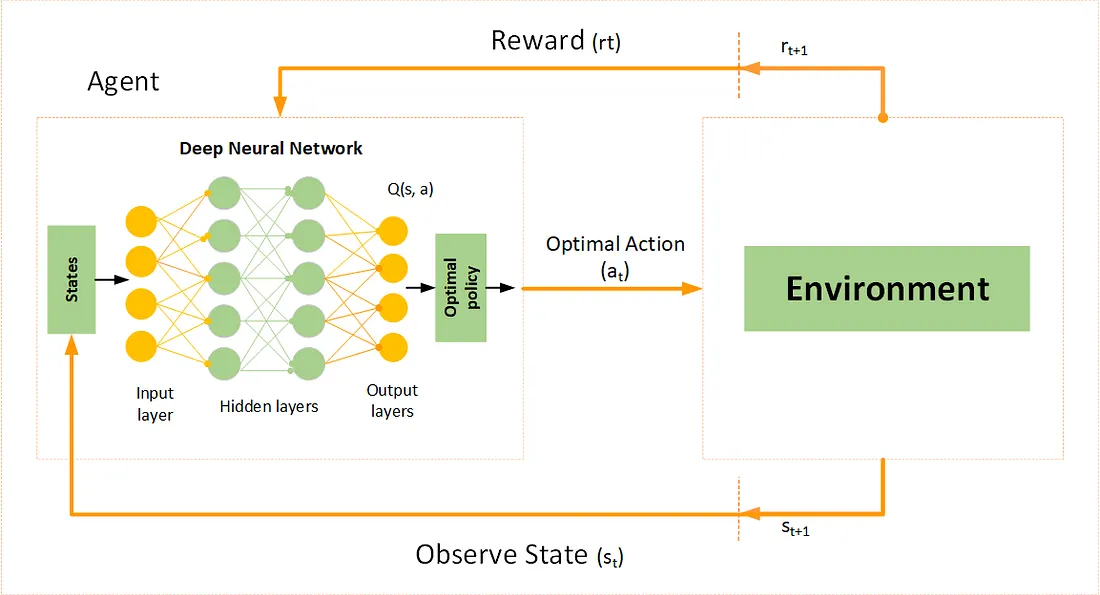
\includegraphics[width=0.9\linewidth,alt={Architecture of the Deep Q-Network}]{figure/dqn} 

}

\caption{DQN Model Architecture}\label{fig:dqn}
\end{figure}

\footnote{Figure \ref{fig:dqn} Retrieved from \url{https://medium.com/@samina.amin/deep-q-learning-dqn-71c109586bae}}

\subsection{Training}\label{training}

The hyperparameters that we set for the first training session are the learning rate (\(\alpha\)), discount factor (\(\gamma\)), and epsilon (\(\epsilon\)) along with its decay and minimum, and batch size.
During our training we will be using the epsilon-greedy policy, where \(\epsilon\) is the probability of a random action being selected and \(1-\epsilon\) is the probability of the highest Q-value action being selected.

The random action chance starts at 1 and will decrease by a factor of 0.995 every episode until it reaches a minimum of 0.01.
The learning rate is initialized to 0.0001, as a sufficiently small learning rate enables the convergence of a Q-value.
Discount factor is initialized to 0.95 to help ensure convergence and the long-term reward maximizing strategy while keeping the computational time low. After each training session we will adjust the hyperparameters based on the model's performance.

Batch size is the number of random samples from the experience replay buffer that will be used to update the network's Q-values.
It is initialized to 16, as it provides low computational time while maintaining good accuracy from during training.
The experience replay buffer is the space where each turn is stored, that is the collection of a state, the action, its reward, and the next state.
We set this to have a maximum size of 1000, so 16 random samples will be selected from here to update the Q-values.

During the training period, the DQN is trained against the decent and advanced level players, as well as the random player. One episode will represent a single game, or simulation.
The opponent is selected randomly for each simulation.
For each episode, the overall win rate, win rate against each individual opponent, epsilon value, reward, Q-value, Q-value loss, and average rule of 28 points are recorded to a CSV (comma-separated values) file for analysis.

This analysis will be looking at these recorded values to find insights into possible strategies.
This includes looking at the players the DQN has the best and worst win rates against to infer where its strengths and weaknesses lie.
Looking at the reward value over time we will analyze the point at which it begins to make choices in an attempt to maximize the reward.
Analyzing the overall win rate will inform us of the accuracy of the model, being able to see when the accuracy plateaus.
Along with accuracy we can see the mean squared error for the Q-values, giving us more insight into the model's performance.

\newpage

\section{Analysis and Results}\label{ana-res}

\subsection{Introduction}\label{introduction}

We trained on 367,029 simulations split between 18 different training sessions, with a different number of games per training session. The simulations were segmented due to time and hardware constraints. Before each run, the hyperparameters were adjusted based on the previous run's results and the target number of simulations. The goal when tuning the hyperparameters was to guide the algorithm towards our research objective of creating a successful Can't Stop computer algorithm. The hyperparameters that had the most changes are the discount factor and epsilon minimum and decay. Discount factor controls the model's predicted Q-values and therefore the play style, where decreasing it reduces predicted Q-values. Epsilon decay determines the rate at which our model will transition from random actions to strategic actions, and the minimum is the smallest chance for the model to make random decisions that we are satisfied with. The raw data is available for download from the Github repository linked in Appendix \ref{ApdxCode}.

\subsection{Predicted vs Actual Q-values}\label{predicted-vs-actual-q-values}

We will start evaluating the model's performance by comparing the predicted Q-values to the rewards (actual Q-values) across each episode. Due to the high volume of data points, we smooth the data using the moving average technique with 500 games to reduce the noise in the data. This makes the visualization of the data easier to see and interpret.

\begin{table}[H]
\centering
\caption{\label{tab:AvgQval}Average Predicted and Actual Q-values}
\centering
\begin{tabular}[t]{r|r|r}
\hline
Run & Avg Reward & Avg Q-value\\
\hline
1 & 0.3795799 & 32.111841\\
\hline
2 & 1.2657258 & 65.580151\\
\hline
3 & 1.2009576 & 63.633910\\
\hline
4 & 1.0417931 & 67.565296\\
\hline
5 & 1.3025428 & 65.427201\\
\hline
6 & 0.3447525 & 41.702243\\
\hline
7 & 0.9572993 & 51.280556\\
\hline
8 & 0.5917869 & 52.834164\\
\hline
9 & 0.4691523 & 60.608044\\
\hline
10 & 1.6260889 & 80.384007\\
\hline
11 & 1.5660336 & 74.550757\\
\hline
12 & 0.8143716 & 4.835290\\
\hline
13 & 0.4656085 & 4.294338\\
\hline
14 & 1.1434122 & 7.277142\\
\hline
15 & 1.0963587 & 6.723077\\
\hline
16 & 1.0406109 & 7.017006\\
\hline
17 & 1.0840146 & 4.967744\\
\hline
18 & 1.1788660 & 5.358426\\
\hline
\end{tabular}
\end{table}

\begin{figure}

\includegraphics[alt={Graphs of runs one through three showing predicted and actual Q-values}]{thesis_files/figure-latex/rewardandq1-1} \caption{Runs 1-3 Rewards vs Predicted Q-values (smoothed)}\label{fig:rewardandq1}
\end{figure}

\begin{figure}

\includegraphics[alt={Graphs of runs four through six showing predicted and actual Q-values}]{thesis_files/figure-latex/rewardandq2-1} \caption{Runs 4-6 Rewards vs Predicted Q-values (smoothed)}\label{fig:rewardandq2}
\end{figure}

\begin{figure}

\includegraphics[alt={Graphs of runs seven through nine showing predicted and actual Q-values}]{thesis_files/figure-latex/rewardandq3-1} \caption{Runs 7-9 Rewards vs Predicted Q-values (smoothed)}\label{fig:rewardandq3}
\end{figure}

\begin{figure}

\includegraphics[alt={Graphs of runs ten through twelve showing predicted and actual Q-values}]{thesis_files/figure-latex/rewardandq4-1} \caption{Runs 10-12 Rewards vs Predicted Q-values (smoothed)}\label{fig:rewardandq4}
\end{figure}

\begin{figure}

\includegraphics[alt={Graphs of runs thirteen through fiftheen showing predicted and actual Q-values}]{thesis_files/figure-latex/rewardandq5-1} \caption{Runs 13-15 Rewards vs Predicted Q-values (smoothed)}\label{fig:rewardandq5}
\end{figure}

\begin{figure}

\includegraphics[alt={Graphs of runs sixteen through eighteen showing predicted and actual Q-values}]{thesis_files/figure-latex/rewardandq6-1} \caption{Runs 16-18 Rewards vs Predicted Q-values (smoothed)}\label{fig:rewardandq6}
\end{figure}

\subsubsection{Observations and Analysis}\label{observations-and-analysis}

Figures \ref{fig:rewardandq1}-\ref{fig:rewardandq6} contain results for the eighteen runs. We can see an overall issue with the model overestimating the Q-values during each training session. While the Q-values are increasing over the training period, the reward remains near zero, not matching the Q-values growth. This means the model is overestimating the quality of its choices each game.

\begin{table}[H]
\centering
\caption{\label{tab:parametertable}Parameter Values}
\centering
\begin{tabular}[t]{r|r|r|r|r|r}
\hline
Run & Simulation Size & Learning Rate & Discount Factor & Epsilon Decay & Epsilon Minimum\\
\hline
1 & 10000 & 0.0001 & 0.95 & 0.99500 & 0.01\\
\hline
2 & 20000 & 0.0001 & 0.95 & 0.99990 & 0.01\\
\hline
3 & 25000 & 0.0001 & 0.95 & 0.99990 & 0.01\\
\hline
4 & 40000 & 0.0001 & 0.95 & 0.99990 & 0.01\\
\hline
5 & 25000 & 0.0001 & 0.95 & 0.99990 & 0.01\\
\hline
6 & 25000 & 0.0001 & 0.95 & 0.99500 & 0.01\\
\hline
7 & 20000 & 0.0001 & 0.95 & 0.99955 & 0.01\\
\hline
8 & 10000 & 0.0001 & 0.95 & 0.99500 & 0.01\\
\hline
9 & 20000 & 0.0001 & 0.95 & 0.99950 & 0.01\\
\hline
10 & 20000 & 0.0001 & 0.95 & 0.99950 & 0.30\\
\hline
11 & 20000 & 0.0001 & 0.95 & 0.99950 & 0.30\\
\hline
12 & 15000 & 0.0001 & 0.50 & 0.99950 & 0.10\\
\hline
13 & 20000 & 0.0001 & 0.50 & 0.99950 & 0.10\\
\hline
14 & 20000 & 0.0001 & 0.50 & 0.99950 & 0.30\\
\hline
15 & 20000 & 0.0001 & 0.50 & 0.99950 & 0.30\\
\hline
16 & 20000 & 0.0001 & 0.50 & 0.99950 & 0.30\\
\hline
17 & 20000 & 0.0001 & 0.30 & 0.99950 & 0.30\\
\hline
18 & 20000 & 0.0001 & 0.30 & 0.99950 & 0.30\\
\hline
\end{tabular}
\end{table}

The first run was 10,000 simulations, with \(\alpha=0.0001\), \(\gamma=0.95\), and \(\epsilon\) decay and minimum set to 0.995 and 0.01 respectively. We can see the overestimation immediately, which could be due to the beginning stages of training where the model is playing the game for the very first time.
For the second and third run, the number of simulations was increased to 20,000 and 25,000 respectively. Since the training periods will be longer the \(\epsilon\) decay is changed to 0.9999 for a slower decay which will allow the model to spend more time exploring new strategies. There is a small increase in the reward value across the training period, implying the model is slowly learning.

The fourth training session was 40,000 simulations with the same hyperparameter values as the previous run. The length of the run was increased in an attempt to reduce the overestimating issue by giving the model a longer training session. As seen in Figure \ref{fig:rewardandq2} above, increasing the simulations did not have a noticeable effect in reducing the Q-value overestimation. The fifth and sixth training sessions were both 25,000 simulations. The sixth session was cut short at 22,029 games due to the training not finishing in the amount of time available. The training taking too long is possibly due to the decrease of the \(\epsilon\) decay to 0.995 causes the model to spend more time exploring. The reward values during the fifth session are the highest overall with an average of 1.302.
The sixth session's \(\epsilon\) decay was set to 0.995 to see if a shorter exploration period would affect the overestimation. While the predicted value peak was lower than previous runs, the reward values were still very low.

For the seventh training session, the number of simulations was reduced to 20,000 and the \(\epsilon\) decay was set to 0.99955. For the eighth training run, the number of simulations was again reduced to 10,000 and \(\epsilon\) decay was set to 0.995. The peak of the predicted values was lower, hanging around 60. For the ninth training, the simulations were returned to 20,000 and \(\epsilon\) decay was set to 0.9995. Interestingly the model reached the plateau of its predicted Q-values sooner than any other training session.

The tenth and eleventh training session had similar results to run 9. The \(\epsilon\) minimum was raised to 0.3 to reduce the model falling into overestimating bad strategies. However, session 10 and 11 had an average reward of 1.626 and 1.566 respectively. This implies the gap between the predicted and actual values is getting smaller. This could be because enough training time has passed for the model to start learning the game. For the twelfth training session the simulation number was reduced to 15,000 and \(\epsilon\) minimum was set to 0.1, and most significantly the discount factor was reduced to 0.5 to encourage short term reward seeking behavior. As seen in Figure \ref{fig:rewardandq4}, there was a larger decrease in the overestimation, with the predicted values getting closer to the actual values as the model finished training.

The next three training sessions are run with almost the same parameters as session 12 to see if the decreased discount will improve the win rate. The \(\epsilon\) minimum was set to 0.3 for 14 and 15 to encourage more learning exploration. As seen in Figure \ref{fig:rewardandq5} and Table \ref{tab:AvgQval}, the overestimation continues to be reduced. The average reward values increase with the predicted values in sessions 14 and 15. We can see that reducing the discount factor did reduce the overestimation as predicted. The model making short term decisions appears to be increasing the quality of the model's training.

Session 16's rewards are similar to session 15 with slightly larger predicted values. For session 17, the discount factor was reduced to 0.3 because of the lack of improvement from session 15 to 16 to see if an even smaller discount factor would decrease the difference between the reward and predicted values. This did cause session 17 to have lower overall values, and when the reward and predicted values increase in session 18 the difference between the values increases as well.

\subsubsection{Conclusion}\label{conclusion}

Looking at the predicted vs actual Q-values to determine our models performance, we can see that it was not as successful as we had hoped with the high discount factor. There was a large presence of overestimation in the predicted values, which seemed to slow the model's training process. However, upon reducing the discount factor we saw an immediate reduction in overestimation. This reduction remains present through the rest of the training. Starting training with the model prioritizing long term rewards can cause the model to chase larger Q-values that are unattainable. The model learned to make decisions that it incorrectly predicted will lead to high rewards while in practice it was making poor decisions. This leads to the large difference seen between the predictions and actual values, the model learned to overestimate the quality of its decisions. Since a Can't Stop game is on the shorter side, typically 8-10 turns per player, the higher discount factor is trying to find rewards for a large number of turns that likely won't be reached.
Starting the training process with a decreased discount factor and increasing it as the model performance increases could lead to a better overall performance of the model in a shorter training period. Different small discount factor values could be experimented with to see which one best fits the Can't Stop play style.

\subsection{Opponent Win Rates}\label{opponent-win-rates}

Looking at the model's win rate, we will analyze how its performance changes across each training session. Also, we look at how it performs against the individual strategies to find the models weaknesses and strengths.

\begin{figure}

\includegraphics[alt={Model's Overall win rate}]{thesis_files/figure-latex/overall-1} \caption{Overall Win Rate per Training Session}\label{fig:overall}
\end{figure}

\begin{figure}

\includegraphics[alt={Model's win rate against the Random Player}]{thesis_files/figure-latex/vsRandom-1} \caption{Versus Random Win Rate per Training Session}\label{fig:vsRandom}
\end{figure}

\begin{figure}

\includegraphics[alt={Model's win rate against the Rule of 28 player and smart Rule of 28 player}]{thesis_files/figure-latex/vsRo28-1} \caption{Versus Ro28 and Smart Ro28 Win Rate per Training Session}\label{fig:vsRo28}
\end{figure}

\begin{figure}

\includegraphics[alt={Model's win rate against the decent Cautious player and advanced Cautious player}]{thesis_files/figure-latex/vsCaut-1} \caption{Versus Cautious Players Win Rate per Training Session}\label{fig:vsCaut}
\end{figure}

\begin{figure}

\includegraphics[alt={Model's win rate against the decent aggressive player and advanced aggressive player}]{thesis_files/figure-latex/vsAggr-1} \caption{Versus Aggressive Players Win Rate per Training Session}\label{fig:vsAggr}
\end{figure}

\subsubsection{Observations and Analysis}\label{observations-and-analysis-1}

As shown in Figure \ref{fig:overall}, the win rate increases from training session 1 to 2, as we would expect and want to see. It then fluctuates before noticeably dropping at training session 6. The win rate decrease was likely a result of changing the \(\epsilon\) decay to 0.995, which caused the model to quickly stop exploring new strategies during training. For the following training sessions the win rate slightly fluctuates and then increases into the end of the training. Although the discount factor was decreased for training session 12, compared to 10 and 11 it does not appear to have made a noticeable impact on the win rate. For sessions 13 and 14, the win rate does not increase staying the same \(5.2\%\). Session 15 has a minor increase to almost \(6\%\). The continued training with the decreased discount factor likely has led to this win rate increase. However, for session 16 the win rate drops down to before, similar to 13 and 14. Session 17 the discount was decreased further, which had a positive effect on the win rate, looking like session 15. However, going into session 18 with the same parameters the win rate dropped. This could be a natural fluctuation in the training process.

Using the random player as a baseline for the model's performance, we hope to see the model be able to perform better than random actions. However, as seen in Figure \ref{fig:vsRandom} it did not perform as well as we hoped. However, compared to the other individual player win rates the model had the highest win rate against the random player for every training session. The increases and decreases follow the overall win rate trend. The second training had the highest win rate out of the 12 training sessions. The win rate seems to be reacting to the change in \(\epsilon\) decay. When the decay is changed to be faster in a longer training session, we see a major decrease of 27\% to 7\%. This is supported by session 10, where the win rate is above 20\% for the first time since session 5. As stated previously, the \(\epsilon\) minimum was decreased to 0.3, which has a similar effect to slowing the decay. This keeps the model in the exploration stage longer. In session 12 the impact of the decreased discount factor is more visible, the decrease forces the model to make more short term choices so we expect a slight performance decrease. While session 13 dips a little, we see a big rise through session 14 and 15. Session 16 drops to a similar win rate as session 14. From this drop the discount factor is decreased to 0.3 to improve win rates, which we see in session 17's increase. Session 18's win rate drops, not continuing session 17's increase.

The Rule of 28 is one the best performing strategies in practice. Our model's performance is seen in Figure \ref{fig:vsRo28}. The model's performance against the pure Ro28 player was the second highest individual win rate during the training. The win rate follows the same overall trend as seen earlier, a rise in the beginning that falls in session 6 followed by a final rise. Comparing the win rate to the smart Ro28, we see a noticeable decrease in performance. Since one of the models inputs was its Ro28 score, this possibly gave it an advantage over the pure strategy. However, introducing more advanced decisions put our model at a disadvantage. Though the win rate against the smart Ro28 stays at \(\approx1\%\), in the last training session we see an increase to almost 3\%. This could correlate with the decrease in the discount factor, the model being able to make more short sighted decisions gives it an advantage over the strategy's complex decision-making algorithm. For the pure Ro28, sessions 13, 15, 16, and 17 all have similar win rates to 12, implying the discount factor decrease is responsible for improving model performance. Session 14 has a slight dip, which is likely an outlier due to a lower number of matches against the Ro28 player. Against the smart Ro28 player, the performance of session 13 follows 12 but it dips back down for sessions 14 though 18.

Figure \ref{fig:vsCaut} tells us the model did poorly against both levels of the cautious strategies. The model did slightly better against the decent level than the advanced level, but not by much. For session 13 against the decent level we see a spike, with the highest win rate of \(\approx4\%\). Looking ahead to Figure \ref{fig:vsAggr}, the outcome of the model's performance against the aggressive players follows a similar trend of low performance with a spike at session 13 against the decent level. The spike at session 13 could be due to a good luck streak for the model or a low amount of matches. This suggests our model's weakness were these more complex decision-focused strategies. The factors these strategies consider like opponent positioning put them at a greater advantage.

\subsubsection{Conclusion}\label{conclusion-1}

Looking at the win rates overall and individually, the model did not perform as well as we expected. Despite that we can still gain insight into how the model was developing its own strategy. The model was being held back by a high discount factor, which made it difficult to hone an effective strategy. While giving the model training time with a smaller discount factor did not show the larger growth we desired, the consistency of its performance was much better. More training with a smaller discount factor that gradually increases with the models performance would likely result in a more powerful model. Another alternative is training a new model on a low and slowly increasing discount factor to ensure it only learns short term reward behavior to start. As well, more time in the early training stage with a high \(\epsilon\) would allow the model to explore and find more unique strategies. The model appeared to have been developing a working strategy, as it was a noticeable amount of games against the random player. The only non-random player the model showed some success against was pure Ro28. Similar to the pure Ro28, the models weakness was the complex decision making which included consideration of opponents progress. This implies the model's strategy was similar to Ro28, sharing a similar weakness.

\subsection{Feature Importance}\label{feature-importance}

For testing the importance of each feature, we use the permutation feature importance method. This method tests the model's features by randomizing a feature's values, then recording the model's win rate. We will use the win rate against the Rule of 28 player as our baseline to compare when testing the randomized feature values. For each feature, they will be permuted for 200 games with the win rate being recorded. The baseline win rate against the Rule of 28 player was \(5.5\%\), so the change in win rate percentage is measured as the difference between the baseline and permuted win rate. The results are shown in Table \ref{tab:featuretable}, ordered from most to least important. The features with a negative percent change indicates the model performed better with the feature permuted compared to the base line.

\begingroup\fontsize{8}{10}\selectfont

\begin{longtable}[t]{r|l|r|r}
\caption{\label{tab:featuretable}Permutation Feature Importance}\\
\hline
Ranking & Feature & Permutated Win Rate & Win Rate \% Change\\
\hline
1 & column\_completed\_this\_turn & 0.010 & 4.5\\
\hline
2 & temp\_marker\_col\_7 & 0.015 & 4.0\\
\hline
3 & opp\_progress\_col\_7 & 0.025 & 3.0\\
\hline
4 & my\_completed\_count & 0.025 & 3.0\\
\hline
5 & opp\_progress\_col\_5 & 0.030 & 2.5\\
\hline
6 & completed\_col\_9 & 0.030 & 2.5\\
\hline
7 & opp\_completed\_count & 0.030 & 2.5\\
\hline
8 & temp\_marker\_col\_8 & 0.035 & 2.0\\
\hline
9 & completed\_col\_2 & 0.035 & 2.0\\
\hline
10 & completed\_col\_11 & 0.035 & 2.0\\
\hline
11 & opp\_progress\_col\_8 & 0.040 & 1.5\\
\hline
12 & temp\_marker\_col\_10 & 0.040 & 1.5\\
\hline
13 & completed\_col\_4 & 0.040 & 1.5\\
\hline
14 & completed\_col\_5 & 0.040 & 1.5\\
\hline
15 & num\_temp\_markers & 0.040 & 1.5\\
\hline
16 & my\_progress\_col\_12 & 0.045 & 1.0\\
\hline
17 & completed\_col\_10 & 0.045 & 1.0\\
\hline
18 & completed\_col\_12 & 0.045 & 1.0\\
\hline
19 & success\_probability & 0.045 & 1.0\\
\hline
20 & opp\_progress\_col\_10 & 0.050 & 0.5\\
\hline
21 & temp\_marker\_col\_5 & 0.050 & 0.5\\
\hline
22 & my\_progress\_col\_4 & 0.055 & 0.0\\
\hline
23 & opp\_progress\_col\_11 & 0.055 & 0.0\\
\hline
24 & rolls\_this\_turn & 0.055 & 0.0\\
\hline
25 & opp\_progress\_col\_4 & 0.060 & -0.5\\
\hline
26 & completed\_col\_6 & 0.060 & -0.5\\
\hline
27 & temp\_marker\_col\_3 & 0.065 & -1.0\\
\hline
28 & temp\_marker\_col\_4 & 0.065 & -1.0\\
\hline
29 & completed\_col\_7 & 0.065 & -1.0\\
\hline
30 & completed\_col\_8 & 0.065 & -1.0\\
\hline
31 & my\_progress\_col\_2 & 0.070 & -1.5\\
\hline
32 & my\_progress\_col\_3 & 0.070 & -1.5\\
\hline
33 & my\_progress\_col\_7 & 0.070 & -1.5\\
\hline
34 & my\_progress\_col\_8 & 0.070 & -1.5\\
\hline
35 & my\_progress\_col\_10 & 0.070 & -1.5\\
\hline
36 & opp\_progress\_col\_3 & 0.070 & -1.5\\
\hline
37 & opp\_progress\_col\_12 & 0.070 & -1.5\\
\hline
38 & temp\_marker\_col\_2 & 0.070 & -1.5\\
\hline
39 & temp\_marker\_col\_9 & 0.070 & -1.5\\
\hline
40 & temp\_marker\_col\_11 & 0.070 & -1.5\\
\hline
41 & temp\_marker\_col\_12 & 0.070 & -1.5\\
\hline
42 & completed\_col\_3 & 0.070 & -1.5\\
\hline
43 & my\_progress\_col\_6 & 0.075 & -2.0\\
\hline
44 & my\_progress\_col\_11 & 0.075 & -2.0\\
\hline
45 & opp\_progress\_col\_2 & 0.080 & -2.5\\
\hline
46 & opp\_progress\_col\_9 & 0.085 & -3.0\\
\hline
47 & my\_progress\_col\_5 & 0.090 & -3.5\\
\hline
48 & opp\_progress\_col\_6 & 0.090 & -3.5\\
\hline
49 & temp\_marker\_col\_6 & 0.090 & -3.5\\
\hline
50 & ro28\_points & 0.105 & -5.0\\
\hline
51 & my\_progress\_col\_9 & 0.110 & -5.5\\
\hline
\end{longtable}
\endgroup{}

\subsubsection{Observations and Analysis}\label{observations-and-analysis-2}

Looking at the table, we see that columns\_completed\_this\_turn, temp\_marker\_column\_7, opp\_progress\_column\_7, and my\_completed\_count showed the highest decrease in performance when permuted. We expect columns\_completed\_this\_turn feature to be important since having correct information about your progress during your turn is an essential part of the game. The model was likely stopping upon completing a column to secure progress, a very common strategy which is usually a good choice. The second most important feature, temp\_marker\_column\_7, implies the model had realized that column 7 was the most likely to be rolled and focused on winning that column. This is supported by the next important feature opp\_progress\_column\_7, which is the model gauging if they are going to lose column 7 to the opponent. The model has learned to prioritize winning column 7 before the opponent. The my\_completed\_count feature means the model was making decisions based on how close it was to winning, and we can see in with the \(7^{th}\) ranked opp\_completed\_count that the model learned to change its decision making based on how close it was to winning or losing. Looking at the features with a negative percent change, my\_progress\_col\_9 had the biggest difference at \(-5.5\). This possibly implies that the model could have learned a bad strategy involving column 9. Randomizing the value could have caused the model to play better by accident or the feature was redundant and a different feature was already capturing the trend of column 9. Another possibility could be related to my\_progress\_col\_5, which also had a very low score. It's possible the model learned that these two columns were not worth going for, as they both have equal probability of being rolled. If we compare the probability of getting 5 or 9 to their column height, it could be a disadvantage to try and win these columns. This pattern is not seen with any other symmetric columns, so it could be unique to 5 and 9. Interestingly the Rule of 28 points feature also recorded a \(5\%\) win rate increase when permuted. The model likely learned a bad understanding of the Rule of 28, so randomizing the values helped it perform better essentially ignoring it. As well since it was going against the actual Rule of 28 player, it was more successful not using the feature it did not understand against a strategy that did.

\subsubsection{Conclusion}\label{conclusion-2}

From the feature importance analysis, we can see the model developed both helpful and unhelpful strategies during its training. As we would expect, the model developed a strategy involving using the columns completed during a turn and completed columns overall. As well the model was using the opponent's completed column count, implying the model had learned to change the play style based on how close it or the opponent was to winning. This is a very helpful play style that likely was behind the winning games during training. As well the model learned to differentiate the value between columns, as it prioritizes column 7 over all the others. Focusing on these features in future training might improve the models performance. This most likely came naturally from the fact 7 has the highest probability of being rolled. The Rule of 28 points feature's lack of importance implies the model might perform better if trained without the feature, instead it might be better to add later into the training process. Many features had little to no impact on the performance, so reducing the features to be less redundant could improve the performance in future training.

\newpage

\section{Conclusion}\label{conclusion-3}

We trained a Deep Q-Network to learn and play Can't Stop. However, the DQN was not successful at playing the game well as it failed to meet the performance baseline. We expected the DQN to win a majority of games against the random player, however we saw a \(21.4\%\) average win rate. There are many possibilities as to why the model failed to meet the performance baseline, such as poor hyperparameter tuning, an over complicated training environment, or using an ineffective learning algorithm.

The main problem seen during the training process was overestimation of the reward values. This was caused by setting the discount factor too high, forcing the model to chase and overestimate long term rewards unachievable in a typical game. While this was adjusted for the last \(3^{rd}\) of the training, as seen in Figures \ref{fig:rewardandq4}-\ref{fig:rewardandq6}, the win rate did not experience enough of an impact. This is likely because the amount of time spent training with the parameter set too high could not be offset with the amount of total training time left. The model spent majority of its time trying to do a futile task, and this likely led to the model creating bad connections with its features. The majority of the model's core knowledge is learned in the initial training stages, so spending that crucial training time learning a very ineffective strategy was a significant hindrance on the model's performance.

The training environment we created involved the model playing games against 7 different playstyles at random to prevent the model from overfitting a hyperspecific strategy. This possibly had the opposite effect as the strategy the model developed was not successful against any playstyle. Training against one or two approaches and the baseline could create a better performing model, with the other playstyles being used for testing only to evaluate the model.
Along with a difficult learning environment, reducing the number of features could also improve the model's performance. Since many of the features had no impact or a negative impact on the performance, reducing the features could allow the model to concentrate on a smaller set of features. Another alternative is to use an ensemble learning technique, either bagging or boosting. From James, Witten, Hastie, and Tibshirani (2021), bagging is taking many subsets of the training data (or features), and build separate models for each set, and combine the outputs to make a prediction. Boosting is similar except the separate models are added sequentially into the main model. Both methods reduce the variance and overfitting bias in the model.

With time, the model could be retrained using a smaller discount factor that increases with performance. Since Can't Stop is a shorter game, models could benefit from a smaller discount factor. Another possible parameter change for future training is increasing the learning rate, which was not able to be tested during this analysis. Increasing the step-size could reduce training time and improve performance as the model uses new information more quickly. Along with these changes to the parameters, reducing the scope of the training environment with less playstyles would be tested. Giving the model a simpler environment to train against could be similar in the approach of studying the toy versions of games to find strategies. The overestimation seen in this analysis is a common issue with training DQN models, so a recent solution is the Double Q-learning algorithm proposed by Van Hasselt, Guez, and Silver (2016). This works by giving the model two Q-tables, one for q-values of the best action choice and the other to evaluate the q-value of the action from the first table. This implementation reduces overestimation however is more computationally expensive compared to standard Q-learning. As discussed above, using the bagging method could also help the model develop the features better.
With more time and computing power, future work using the double Q-learning method with bagging, reducing the training environment, and better parameterization could produce a better performing model with a unique strategy to analyze and learn from.

\newpage

\section*{References}\label{references}
\addcontentsline{toc}{section}{References}

\markboth{References}{References}

\noindent Canakci, B., Serrano, S., Roy, O., and Kruskal, C. (2016), ``The Can't Stop Game'', REU-CAAR 2016, Available at \url{https://www.cs.umd.edu/~gasarch/REU/reupapers.html}.

\noindent Cheong, Y. J. (2020), ``Learning to play Can't Stop with a Deep Q Network'', Author. Available at \url{https://yujia21.github.io/personal/cant-stop.html}.

\noindent Fang, H., Gleen, J., and Kruskal, C. (2008), ``Retrograde Approximation Algorithms for Jeopardy Stochastic Games'', \emph{International Computer Games Association}, 31(2), 77-96. Available at \url{https://doi.org/10.3233/icg-2008-31203}.

\noindent Glenn, J. R., \& Aloi, C. J. (2009), ``A Generalized Heuristic for Can't Stop'', \emph{Proceedings of the Twenty-Second International FLAIRS Conference}, 421-426. Available at \url{https://aaai.org/papers/flairs-2009-123/}.

\noindent James, G., Witten, D., Hastie, T., and Tibshirani, R. (2021), \emph{An Introduction to Statistical Learning} (2nd ed.), New York City, NY: Springer.

\noindent Keller, M. (1986), ``Can't Stop? Try The Rule of 28'', Author, Available at \url{https://www.solitairelaboratory.com/cantstop.html}.

\noindent Packel, E. (2006), \emph{The Mathematics of Games and Gambling} (2nd ed.), Washington, DC: The Mathematical Association of America.

\noindent Rapoport, A. (1966), \emph{Two Person Game Theory}, Garden City, NY: Dover Publications.

\noindent Sutton, R., and Barto, A. (2015), \emph{Reinforcement Learning: An Introduction} (2nd ed.), Cambridge, MA: The MIT Press.

\noindent Tate and Renner (2007), ``Can't Stop Odds'', Author, Available at \url{https://www.taterenner.com/cantstop.php}.

\noindent Tesauro, G. (2002), ``Programming backgammon using self-teaching neural nets'', \emph{Artificial Intelligence}, 134, 181-199, Available at \url{https://doi.org/10.1016/S0004-3702(01)00110-2}.

\noindent Van Hasselt, H., Guez, A., and Silver, D. (2016), ``Deep reinforcement learning with double q-learning'', \emph{Proceedings of the AAAI conference on artificial intelligence}, 30(1), Available at \url{https://doi.org/10.1609/aaai.v30i1.10295}.

\noindent Watkins, C. (1989), \emph{Learning from Delayed Rewards}, Ph.D.~dissertation, King's College London.

\setlength{\parindent}{-0.20in}

\appendix

\section{Appendix: Odds Table}\label{ApdxOdds}

\begin{figure}

{\centering 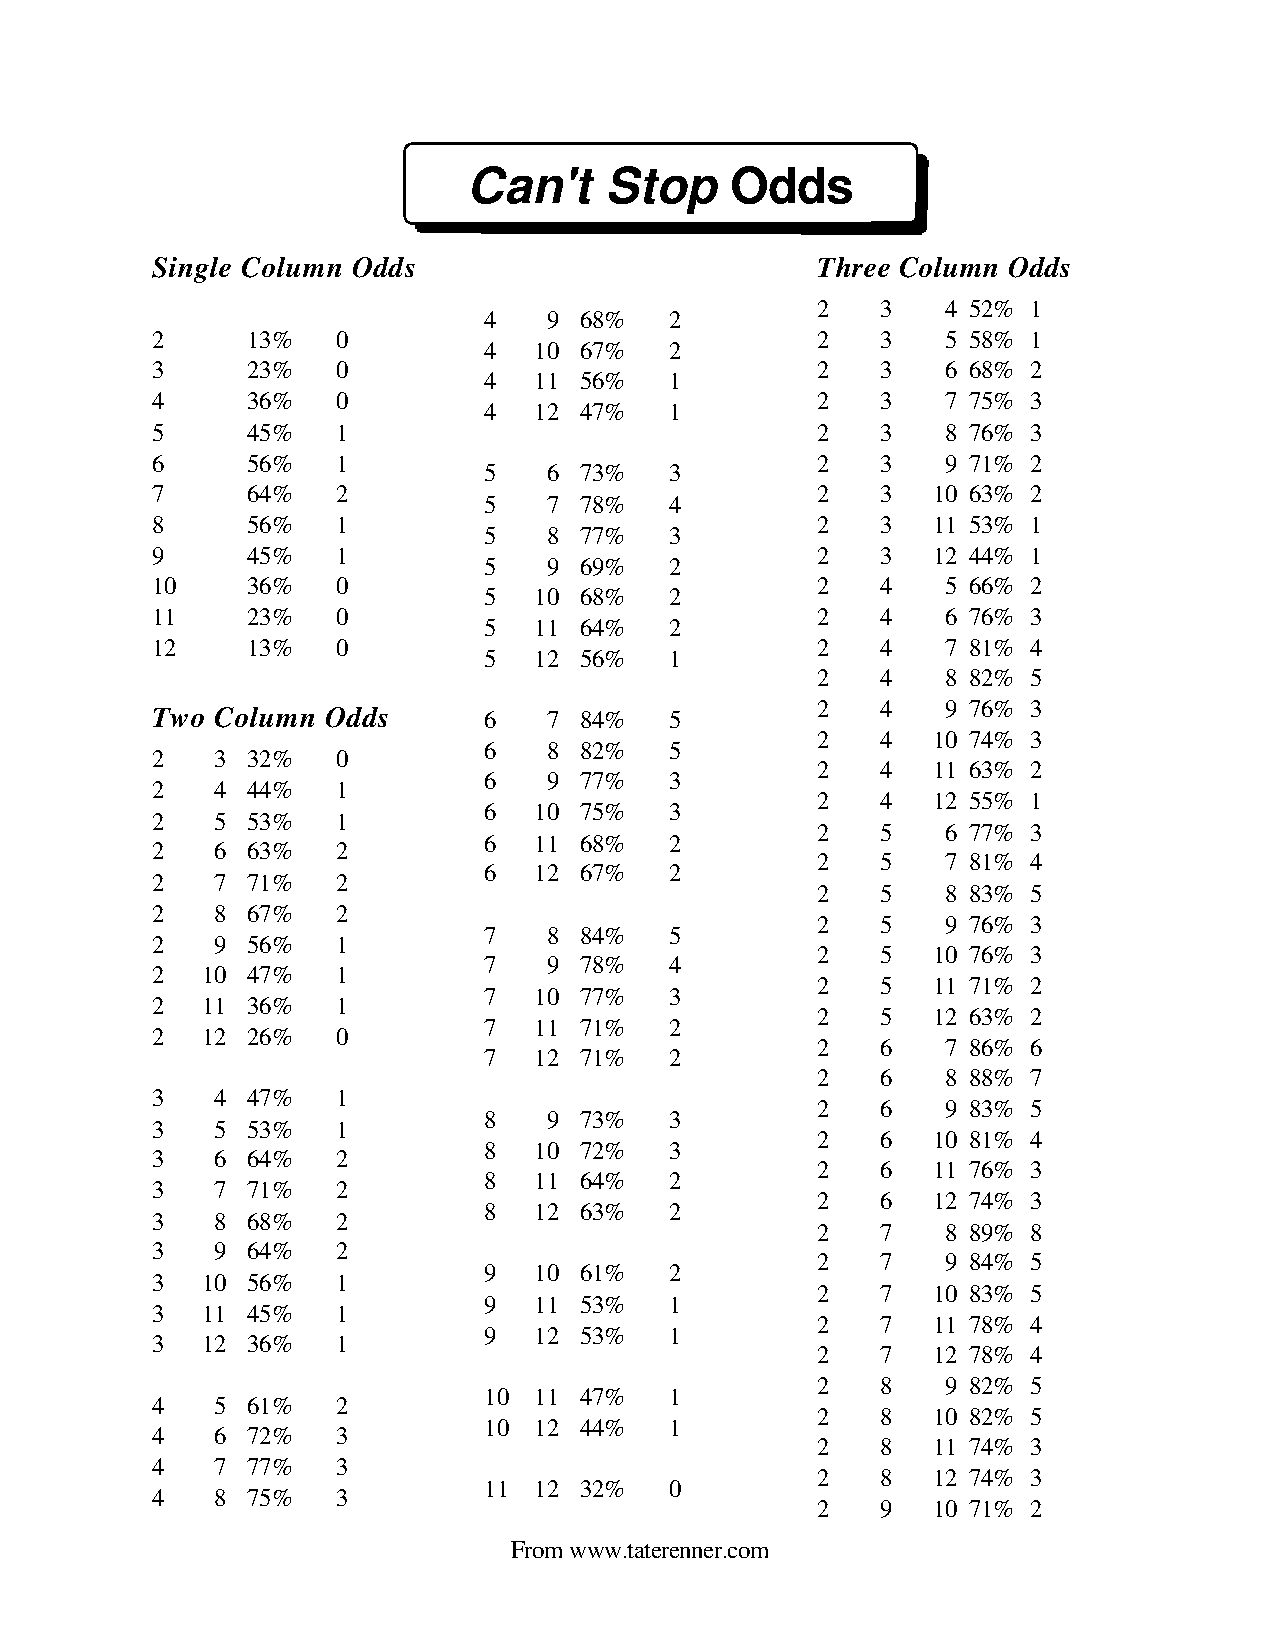
\includegraphics[width=0.9\linewidth]{figure/cantstopodds} 

}

\caption{Can't Stop Odds (Tate and Renner 2007)}\label{fig:oddstable-1}
\end{figure}
\begin{figure}

{\centering 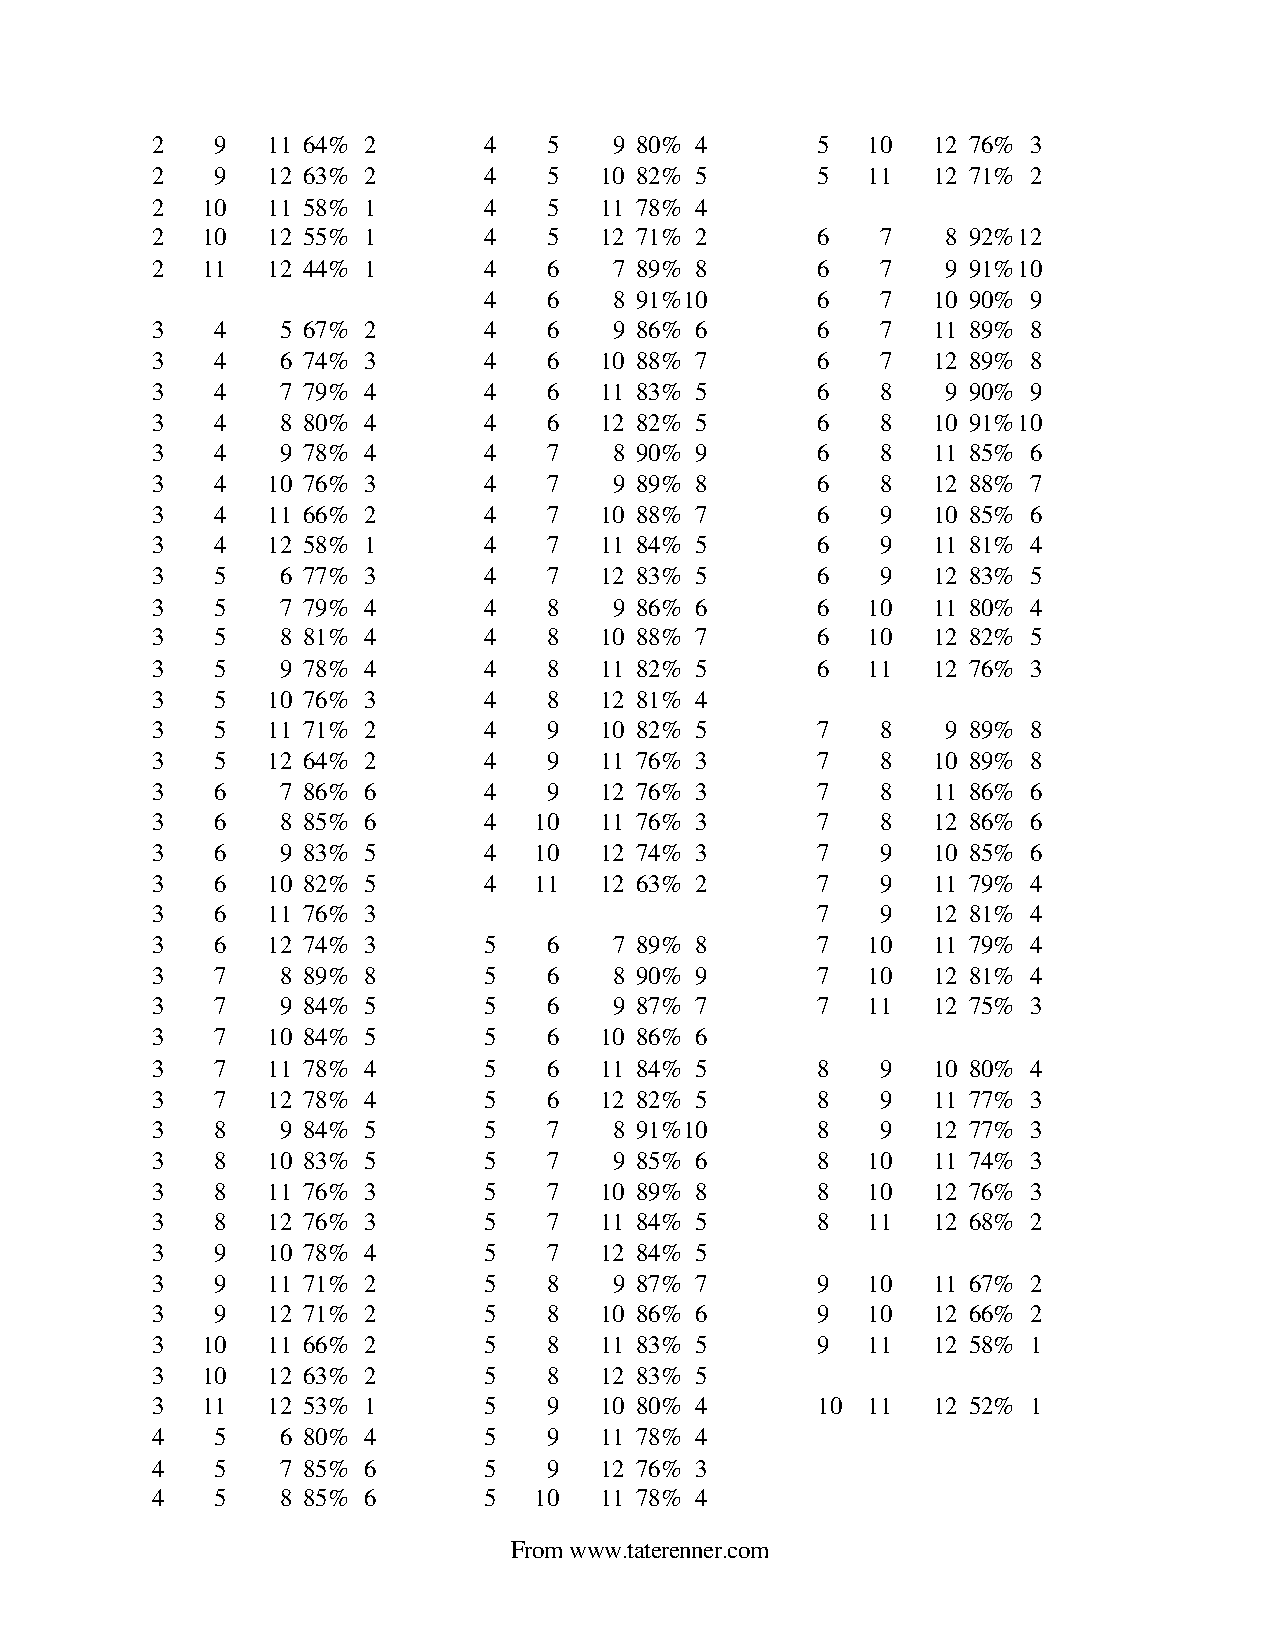
\includegraphics[width=0.9\linewidth]{figure/cantstopoddsp2} 

}

\caption{Can't Stop Odds (Tate and Renner 2007)}\label{fig:oddstable-2}
\end{figure}

\section{Appendix: Python Code \& Github}\label{ApdxCode}

\url{https://github.com/JCameronCarter/HonorsThesis}

\begin{Shaded}
\begin{Highlighting}[]
\ImportTok{import}\NormalTok{ numpy }\ImportTok{as}\NormalTok{ np}
\ImportTok{import}\NormalTok{ random}
\ImportTok{from}\NormalTok{ collections }\ImportTok{import}\NormalTok{ deque}
\ImportTok{import}\NormalTok{ tensorflow }\ImportTok{as}\NormalTok{ tf}
\ImportTok{from}\NormalTok{ tensorflow }\ImportTok{import}\NormalTok{ keras}
\ImportTok{from}\NormalTok{ keras }\ImportTok{import}\NormalTok{ layers}
\ImportTok{from}\NormalTok{ typing }\ImportTok{import}\NormalTok{ List, Tuple, Set}

\CommentTok{\# Import from existing file}
\ImportTok{from}\NormalTok{ CantStop }\ImportTok{import}\NormalTok{ (}
\NormalTok{    CantStopGame, }
\NormalTok{    PlayerStrategy, }
\NormalTok{    RuleOf28,}
\NormalTok{    AdvancedAggressivePlayer}
\NormalTok{)}

\KeywordTok{class}\NormalTok{ DQNPlayer(PlayerStrategy):}
    \CommentTok{\# Deep Q{-}Learning player for Can\textquotesingle{}t Stop}
    
    \KeywordTok{def} \FunctionTok{\_\_init\_\_}\NormalTok{(}\VariableTok{self}\NormalTok{, state\_size}\OperatorTok{=}\DecValTok{51}\NormalTok{, action\_size}\OperatorTok{=}\DecValTok{2}\NormalTok{, }
\NormalTok{                load\_model}\OperatorTok{=}\VariableTok{None}\NormalTok{, training}\OperatorTok{=}\VariableTok{True}\NormalTok{):}
        \VariableTok{self}\NormalTok{.state\_size }\OperatorTok{=}\NormalTok{ state\_size}
        \VariableTok{self}\NormalTok{.action\_size }\OperatorTok{=}\NormalTok{ action\_size}
        \VariableTok{self}\NormalTok{.training }\OperatorTok{=}\NormalTok{ training}
        
        \CommentTok{\# Hyperparameters}
        \VariableTok{self}\NormalTok{.learning\_rate }\OperatorTok{=} \FloatTok{0.0001}
        \VariableTok{self}\NormalTok{.gamma }\OperatorTok{=} \FloatTok{0.3} 
        \VariableTok{self}\NormalTok{.epsilon }\OperatorTok{=} \FloatTok{1.0}
        \VariableTok{self}\NormalTok{.epsilon\_min }\OperatorTok{=} \FloatTok{0.3}
        \VariableTok{self}\NormalTok{.epsilon\_decay }\OperatorTok{=} \FloatTok{0.9995}
        \VariableTok{self}\NormalTok{.batch\_size }\OperatorTok{=} \DecValTok{16}
        
        \CommentTok{\# Experience replay memory}
        \VariableTok{self}\NormalTok{.memory }\OperatorTok{=}\NormalTok{ deque(maxlen}\OperatorTok{=}\DecValTok{1000}\NormalTok{)}
        
        \CommentTok{\# Metric Tracking}
        \VariableTok{self}\NormalTok{.episode\_rewards }\OperatorTok{=}\NormalTok{ []         }
        \VariableTok{self}\NormalTok{.episode\_q\_values }\OperatorTok{=}\NormalTok{ []          }
        \VariableTok{self}\NormalTok{.last\_loss }\OperatorTok{=} \FloatTok{0.0}                
        \VariableTok{self}\NormalTok{.episode\_ro28\_points }\OperatorTok{=}\NormalTok{ []}

        \CommentTok{\# Game state tracking}
        \VariableTok{self}\NormalTok{.rolls\_this\_turn }\OperatorTok{=} \DecValTok{0}
        \VariableTok{self}\NormalTok{.columns\_started\_this\_turn }\OperatorTok{=} \BuiltInTok{set}\NormalTok{()}
        
        \CommentTok{\# Build networks}
        \ControlFlowTok{if}\NormalTok{ load\_model:}
            \VariableTok{self}\NormalTok{.model }\OperatorTok{=}\NormalTok{ keras.models.load\_model(load\_model)}
            \VariableTok{self}\NormalTok{.target\_model }\OperatorTok{=}\NormalTok{ keras.models.load\_model(load\_model)}
        \ControlFlowTok{else}\NormalTok{:}
            \VariableTok{self}\NormalTok{.model }\OperatorTok{=} \VariableTok{self}\NormalTok{.\_build\_model()}
            \VariableTok{self}\NormalTok{.target\_model }\OperatorTok{=} \VariableTok{self}\NormalTok{.\_build\_model()}
            \VariableTok{self}\NormalTok{.update\_target\_model()}
    
    \KeywordTok{def}\NormalTok{ \_build\_model(}\VariableTok{self}\NormalTok{):}
        \CommentTok{\#Build the Q{-}network}
\NormalTok{        model }\OperatorTok{=}\NormalTok{ keras.Sequential([}
\NormalTok{            layers.Dense(}\DecValTok{64}\NormalTok{, activation}\OperatorTok{=}\StringTok{\textquotesingle{}relu\textquotesingle{}}\NormalTok{, }
\NormalTok{            input\_shape}\OperatorTok{=}\NormalTok{(}\VariableTok{self}\NormalTok{.state\_size,)),}
\NormalTok{            layers.Dropout(}\FloatTok{0.2}\NormalTok{),}
\NormalTok{            layers.Dense(}\DecValTok{64}\NormalTok{, activation}\OperatorTok{=}\StringTok{\textquotesingle{}relu\textquotesingle{}}\NormalTok{),}
\NormalTok{            layers.Dropout(}\FloatTok{0.2}\NormalTok{),}
\NormalTok{            layers.Dense(}\VariableTok{self}\NormalTok{.action\_size, activation}\OperatorTok{=}\StringTok{\textquotesingle{}linear\textquotesingle{}}\NormalTok{)}
\NormalTok{        ])}
\NormalTok{        model.}\BuiltInTok{compile}\NormalTok{(optimizer}\OperatorTok{=}\NormalTok{keras.optimizers.}
\NormalTok{                      Adam(learning\_rate}\OperatorTok{=}\VariableTok{self}\NormalTok{.learning\_rate),loss}\OperatorTok{=}\StringTok{\textquotesingle{}mse\textquotesingle{}}\NormalTok{)}
        \ControlFlowTok{return}\NormalTok{ model}
    
    \KeywordTok{def}\NormalTok{ update\_target\_model(}\VariableTok{self}\NormalTok{):}
        \CommentTok{\#Copy weights from model to target\_model}
        \VariableTok{self}\NormalTok{.target\_model.set\_weights(}\VariableTok{self}\NormalTok{.model.get\_weights())}
    
    \KeywordTok{def}\NormalTok{ \_encode\_state(}\VariableTok{self}\NormalTok{, game: CantStopGame) }\OperatorTok{{-}\textgreater{}}\NormalTok{ np.ndarray:}
        \CommentTok{\#Convert game state to feature vector}
\NormalTok{        features }\OperatorTok{=}\NormalTok{ []}
\NormalTok{        current\_player }\OperatorTok{=}\NormalTok{ game.current\_player}
\NormalTok{        opponent\_id }\OperatorTok{=} \DecValTok{1} \OperatorTok{{-}}\NormalTok{ current\_player}
        
        \CommentTok{\# Model\textquotesingle{}s permanent progress (11 values (1 per column), normalized}
        \ControlFlowTok{for}\NormalTok{ col }\KeywordTok{in} \BuiltInTok{range}\NormalTok{(}\DecValTok{2}\NormalTok{, }\DecValTok{13}\NormalTok{):}
\NormalTok{            progress }\OperatorTok{=}\NormalTok{ game.board.player\_markers[current\_player][col]}
\NormalTok{            height }\OperatorTok{=}\NormalTok{ game.board.Column\_Heights[col]}
\NormalTok{            features.append(progress }\OperatorTok{/}\NormalTok{ height)}
        
        \CommentTok{\#Opponent permanent progress (11 values(1 per column), normalized)}
        \ControlFlowTok{for}\NormalTok{ col }\KeywordTok{in} \BuiltInTok{range}\NormalTok{(}\DecValTok{2}\NormalTok{, }\DecValTok{13}\NormalTok{):}
\NormalTok{            progress }\OperatorTok{=}\NormalTok{ game.board.player\_markers[opponent\_id][col]}
\NormalTok{            height }\OperatorTok{=}\NormalTok{ game.board.Column\_Heights[col]}
\NormalTok{            features.append(progress }\OperatorTok{/}\NormalTok{ height)}
        
        \CommentTok{\# Current temp markers (11 values (1 per column), normalized)}
        \ControlFlowTok{for}\NormalTok{ col }\KeywordTok{in} \BuiltInTok{range}\NormalTok{(}\DecValTok{2}\NormalTok{, }\DecValTok{13}\NormalTok{):}
            \ControlFlowTok{if}\NormalTok{ col }\KeywordTok{in}\NormalTok{ game.board.temp\_markers:}
\NormalTok{                temp\_progress }\OperatorTok{=}\NormalTok{ game.board.temp\_markers[col] }\OperatorTok{{-}}
\NormalTok{                          game.board.player\_markers[current\_player][col]}
\NormalTok{                height }\OperatorTok{=}\NormalTok{ game.board.Column\_Heights[col]}
\NormalTok{                features.append(temp\_progress }\OperatorTok{/}\NormalTok{ height)}
            \ControlFlowTok{else}\NormalTok{:}
\NormalTok{                features.append(}\FloatTok{0.0}\NormalTok{)}
        
        \CommentTok{\# Completed columns (11 binary (1 per column))}
        \ControlFlowTok{for}\NormalTok{ col }\KeywordTok{in} \BuiltInTok{range}\NormalTok{(}\DecValTok{2}\NormalTok{, }\DecValTok{13}\NormalTok{):}
\NormalTok{            features.append(}\FloatTok{1.0} \ControlFlowTok{if}\NormalTok{ col }\KeywordTok{in}\NormalTok{ game.board.completed }\ControlFlowTok{else} \FloatTok{0.0}\NormalTok{)}
        
        \CommentTok{\# Number of rolls this turn (1, normalized)}
\NormalTok{        features.append(}\BuiltInTok{min}\NormalTok{(}\VariableTok{self}\NormalTok{.rolls\_this\_turn }\OperatorTok{/} \FloatTok{10.0}\NormalTok{, }\FloatTok{1.0}\NormalTok{))}
        
        \CommentTok{\# Rule of 28 points (1, normalized)}
\NormalTok{        ro28\_points }\OperatorTok{=}\NormalTok{ RuleOf28.calulate\_points(game, }
                                              \VariableTok{self}\NormalTok{.columns\_started\_this\_turn)}
\NormalTok{        features.append(ro28\_points }\OperatorTok{/} \FloatTok{50.0}\NormalTok{)}
        
        \CommentTok{\# Success probability (1)}
\NormalTok{        temp\_cols }\OperatorTok{=} \BuiltInTok{set}\NormalTok{(game.board.temp\_markers.keys())}
        \ControlFlowTok{if} \BuiltInTok{len}\NormalTok{(temp\_cols) }\OperatorTok{==} \DecValTok{3}\NormalTok{:}
\NormalTok{            features.append(game.board.}
\NormalTok{                            get\_success\_probability(game.board.temp\_markers))}
        \ControlFlowTok{else}\NormalTok{:}
\NormalTok{            features.append(}\FloatTok{1.0}\NormalTok{)}
        
        \CommentTok{\# Number of temp markers (1, normalized)}
\NormalTok{        features.append(}\BuiltInTok{len}\NormalTok{(game.board.temp\_markers) }\OperatorTok{/} \FloatTok{3.0}\NormalTok{)}
        
        \CommentTok{\# Model\textquotesingle{}s completed columns (1)}
\NormalTok{        my\_completed }\OperatorTok{=} \BuiltInTok{sum}\NormalTok{(}
            \DecValTok{1} \ControlFlowTok{for}\NormalTok{ col }\KeywordTok{in}\NormalTok{ game.board.completed}
            \ControlFlowTok{if}\NormalTok{ game.board.player\_markers[current\_player][col] }\OperatorTok{\textgreater{}=} 
\NormalTok{                                              game.board.Column\_Heights[col]}
\NormalTok{        )}
\NormalTok{        features.append(my\_completed }\OperatorTok{/} \FloatTok{3.0}\NormalTok{)}
        
        \CommentTok{\# Opponent completed columns (1)}
\NormalTok{        opp\_completed }\OperatorTok{=} \BuiltInTok{sum}\NormalTok{(}
            \DecValTok{1} \ControlFlowTok{for}\NormalTok{ col }\KeywordTok{in}\NormalTok{ game.board.completed}
            \ControlFlowTok{if}\NormalTok{ game.board.player\_markers[opponent\_id][col] }\OperatorTok{\textgreater{}=} 
\NormalTok{                                              game.board.Column\_Heights[col]}
\NormalTok{        )}
\NormalTok{        features.append(opp\_completed }\OperatorTok{/} \FloatTok{3.0}\NormalTok{)}
        
        \CommentTok{\# Any column completed this turn? (1)}
\NormalTok{        completed\_this\_turn }\OperatorTok{=} \BuiltInTok{any}\NormalTok{(}
\NormalTok{            game.board.temp\_markers.get(col, }\DecValTok{0}\NormalTok{) }\OperatorTok{\textgreater{}=} 
\NormalTok{                                              game.board.Column\_Heights[col]}
            \ControlFlowTok{for}\NormalTok{ col }\KeywordTok{in}\NormalTok{ game.board.temp\_markers.keys()}
\NormalTok{        )}
\NormalTok{        features.append(}\FloatTok{1.0} \ControlFlowTok{if}\NormalTok{ completed\_this\_turn }\ControlFlowTok{else} \FloatTok{0.0}\NormalTok{)}
        
        \ControlFlowTok{return}\NormalTok{ np.array(features, dtype}\OperatorTok{=}\NormalTok{np.float32)}
    
    \KeywordTok{def}\NormalTok{ remember(}\VariableTok{self}\NormalTok{, state, action, reward, next\_state, done):}
        \CommentTok{\#Store experience in replay memory}
        \VariableTok{self}\NormalTok{.memory.append((state, action, reward, next\_state, done))}
    
    \KeywordTok{def}\NormalTok{ act(}\VariableTok{self}\NormalTok{, state):}
        \CommentTok{\#Choose action using epsilon{-}greedy policy}
        \ControlFlowTok{if} \VariableTok{self}\NormalTok{.training }\KeywordTok{and}\NormalTok{ np.random.rand() }\OperatorTok{\textless{}=} \VariableTok{self}\NormalTok{.epsilon:}
            \ControlFlowTok{return}\NormalTok{ random.randrange(}\VariableTok{self}\NormalTok{.action\_size)}
        
\NormalTok{        state }\OperatorTok{=}\NormalTok{ state.reshape(}\DecValTok{1}\NormalTok{, }\OperatorTok{{-}}\DecValTok{1}\NormalTok{)}
\NormalTok{        q\_values }\OperatorTok{=} \VariableTok{self}\NormalTok{.model.predict(state, verbose}\OperatorTok{=}\DecValTok{0}\NormalTok{)}

        \ControlFlowTok{if} \VariableTok{self}\NormalTok{.training:}
            \VariableTok{self}\NormalTok{.episode\_q\_values.append(np.}\BuiltInTok{max}\NormalTok{(q\_values[}\DecValTok{0}\NormalTok{]))}

        \ControlFlowTok{return}\NormalTok{ np.argmax(q\_values[}\DecValTok{0}\NormalTok{])}
    
    \KeywordTok{def}\NormalTok{ replay(}\VariableTok{self}\NormalTok{):}
        \CommentTok{\#Train on a batch of experiences}
        \ControlFlowTok{if} \BuiltInTok{len}\NormalTok{(}\VariableTok{self}\NormalTok{.memory) }\OperatorTok{\textless{}} \VariableTok{self}\NormalTok{.batch\_size:}
            \ControlFlowTok{return}
        
\NormalTok{        minibatch }\OperatorTok{=}\NormalTok{ random.sample(}\VariableTok{self}\NormalTok{.memory, }\VariableTok{self}\NormalTok{.batch\_size)}
        
\NormalTok{        states }\OperatorTok{=}\NormalTok{ np.array([exp[}\DecValTok{0}\NormalTok{] }\ControlFlowTok{for}\NormalTok{ exp }\KeywordTok{in}\NormalTok{ minibatch])}
\NormalTok{        actions }\OperatorTok{=}\NormalTok{ np.array([exp[}\DecValTok{1}\NormalTok{] }\ControlFlowTok{for}\NormalTok{ exp }\KeywordTok{in}\NormalTok{ minibatch])}
\NormalTok{        rewards }\OperatorTok{=}\NormalTok{ np.array([exp[}\DecValTok{2}\NormalTok{] }\ControlFlowTok{for}\NormalTok{ exp }\KeywordTok{in}\NormalTok{ minibatch])}
\NormalTok{        next\_states }\OperatorTok{=}\NormalTok{ np.array([exp[}\DecValTok{3}\NormalTok{] }\ControlFlowTok{for}\NormalTok{ exp }\KeywordTok{in}\NormalTok{ minibatch])}
\NormalTok{        dones }\OperatorTok{=}\NormalTok{ np.array([exp[}\DecValTok{4}\NormalTok{] }\ControlFlowTok{for}\NormalTok{ exp }\KeywordTok{in}\NormalTok{ minibatch])}
        
        \CommentTok{\# Predict Q{-}values}
\NormalTok{        current\_q }\OperatorTok{=} \VariableTok{self}\NormalTok{.model.predict(states, verbose}\OperatorTok{=}\DecValTok{0}\NormalTok{)}
\NormalTok{        next\_q }\OperatorTok{=} \VariableTok{self}\NormalTok{.target\_model.predict(next\_states, verbose}\OperatorTok{=}\DecValTok{0}\NormalTok{)}
        
        \CommentTok{\# Update Q{-}values using Bellman equation}
        \ControlFlowTok{for}\NormalTok{ i }\KeywordTok{in} \BuiltInTok{range}\NormalTok{(}\VariableTok{self}\NormalTok{.batch\_size):}
            \ControlFlowTok{if}\NormalTok{ dones[i]:}
\NormalTok{                current\_q[i][actions[i]] }\OperatorTok{=}\NormalTok{ rewards[i]}
            \ControlFlowTok{else}\NormalTok{:}
\NormalTok{                current\_q[i][actions[i]] }\OperatorTok{=}\NormalTok{ rewards[i] }\OperatorTok{+} 
                                           \VariableTok{self}\NormalTok{.gamma }\OperatorTok{*}\NormalTok{ np.}\BuiltInTok{max}\NormalTok{(next\_q[i])}
        
        \CommentTok{\# Train the model}
\NormalTok{        history }\OperatorTok{=}\VariableTok{self}\NormalTok{.model.fit(states, current\_q, epochs}\OperatorTok{=}\DecValTok{1}\NormalTok{, verbose}\OperatorTok{=}\DecValTok{0}\NormalTok{)}
        
        \VariableTok{self}\NormalTok{.last\_loss }\OperatorTok{=}\NormalTok{ history.history[}\StringTok{\textquotesingle{}loss\textquotesingle{}}\NormalTok{][}\DecValTok{0}\NormalTok{]}

        \CommentTok{\# Decay epsilon}
        \ControlFlowTok{if} \VariableTok{self}\NormalTok{.epsilon }\OperatorTok{\textgreater{}} \VariableTok{self}\NormalTok{.epsilon\_min:}
            \VariableTok{self}\NormalTok{.epsilon }\OperatorTok{*=} \VariableTok{self}\NormalTok{.epsilon\_decay}
    
    \KeywordTok{def}\NormalTok{ reset\_episode\_metrics(}\VariableTok{self}\NormalTok{):}
        \CommentTok{\#Reset metrics at the start of an episode}
        \VariableTok{self}\NormalTok{.episode\_rewards }\OperatorTok{=}\NormalTok{ []}
        \VariableTok{self}\NormalTok{.episode\_q\_values }\OperatorTok{=}\NormalTok{ []}
        \VariableTok{self}\NormalTok{.episode\_ro28\_points }\OperatorTok{=}\NormalTok{ []}

    \KeywordTok{def}\NormalTok{ get\_episode\_metrics(}\VariableTok{self}\NormalTok{):}
        \CommentTok{\#Get metrics for the current episode}
\NormalTok{        avg\_reward }\OperatorTok{=}\NormalTok{ np.mean(}\VariableTok{self}\NormalTok{.episode\_rewards) }
                              \ControlFlowTok{if} \VariableTok{self}\NormalTok{.episode\_rewards }\ControlFlowTok{else} \FloatTok{0.0}
\NormalTok{        avg\_q\_value }\OperatorTok{=}\NormalTok{ np.mean(}\VariableTok{self}\NormalTok{.episode\_q\_values) }
                              \ControlFlowTok{if} \VariableTok{self}\NormalTok{.episode\_q\_values }\ControlFlowTok{else} \FloatTok{0.0}
\NormalTok{        avg\_ro28\_points }\OperatorTok{=}\NormalTok{ np.mean(}\VariableTok{self}\NormalTok{.episode\_ro28\_points) }
                                  \ControlFlowTok{if} \VariableTok{self}\NormalTok{.episode\_ro28\_points }\ControlFlowTok{else} \FloatTok{0.0}
        \ControlFlowTok{return}\NormalTok{ \{}
            \StringTok{\textquotesingle{}avg\_reward\textquotesingle{}}\NormalTok{: avg\_reward,}
            \StringTok{\textquotesingle{}avg\_q\_value\textquotesingle{}}\NormalTok{: avg\_q\_value,}
            \StringTok{\textquotesingle{}loss\textquotesingle{}}\NormalTok{: }\VariableTok{self}\NormalTok{.last\_loss,}
            \StringTok{\textquotesingle{}avg\_ro28\_points\textquotesingle{}}\NormalTok{: avg\_ro28\_points}
\NormalTok{        \}}

    \KeywordTok{def}\NormalTok{ decide\_to\_roll(}\VariableTok{self}\NormalTok{, game: CantStopGame) }\OperatorTok{{-}\textgreater{}} \BuiltInTok{bool}\NormalTok{:}
        \ControlFlowTok{if} \VariableTok{self}\NormalTok{.rolls\_this\_turn }\OperatorTok{==} \DecValTok{0}\NormalTok{:}
            \VariableTok{self}\NormalTok{.columns\_started\_this\_turn }\OperatorTok{=} \BuiltInTok{set}\NormalTok{()}
            \ControlFlowTok{return} \VariableTok{True}
        
\NormalTok{        state }\OperatorTok{=} \VariableTok{self}\NormalTok{.\_encode\_state(game)}
\NormalTok{        action }\OperatorTok{=} \VariableTok{self}\NormalTok{.act(state)}
        
        \CommentTok{\# Store state for later reward calculation}
        \VariableTok{self}\NormalTok{.last\_state }\OperatorTok{=}\NormalTok{ state}
        \VariableTok{self}\NormalTok{.last\_action }\OperatorTok{=}\NormalTok{ action}
        
        \ControlFlowTok{return}\NormalTok{ action }\OperatorTok{==} \DecValTok{1}
    
    \KeywordTok{def}\NormalTok{ choose\_move(}\VariableTok{self}\NormalTok{, game: CantStopGame, valid\_moves: }
\NormalTok{                                List[Tuple[}\BuiltInTok{int}\NormalTok{, }\BuiltInTok{int}\NormalTok{]]) }\OperatorTok{{-}\textgreater{}}\NormalTok{ Tuple[}\BuiltInTok{int}\NormalTok{, }\BuiltInTok{int}\NormalTok{]:}
        \VariableTok{self}\NormalTok{.rolls\_this\_turn }\OperatorTok{+=} \DecValTok{1}
        
        \CommentTok{\# Use heuristics for move selection}
\NormalTok{        temp\_cols }\OperatorTok{=} \BuiltInTok{set}\NormalTok{(game.board.temp\_markers.keys())}
        
        \ControlFlowTok{for}\NormalTok{ move }\KeywordTok{in}\NormalTok{ valid\_moves:}
            \ControlFlowTok{if}\NormalTok{ move[}\DecValTok{0}\NormalTok{] }\KeywordTok{in}\NormalTok{ temp\_cols }\KeywordTok{or}\NormalTok{ move[}\DecValTok{1}\NormalTok{] }\KeywordTok{in}\NormalTok{ temp\_cols:}
                \ControlFlowTok{return}\NormalTok{ move}
        
        \ControlFlowTok{return} \BuiltInTok{min}\NormalTok{(valid\_moves, key}\OperatorTok{=}\KeywordTok{lambda}\NormalTok{ m: }\BuiltInTok{abs}\NormalTok{(m[}\DecValTok{0}\NormalTok{] }\OperatorTok{{-}} \DecValTok{7}\NormalTok{) }\OperatorTok{+} \BuiltInTok{abs}\NormalTok{(m[}\DecValTok{1}\NormalTok{] }\OperatorTok{{-}} \DecValTok{7}\NormalTok{))}


\KeywordTok{class}\NormalTok{ RLTrainer:}
    \CommentTok{\#Training environment for DQN player}
    
    \KeywordTok{def} \FunctionTok{\_\_init\_\_}\NormalTok{(}\VariableTok{self}\NormalTok{, opponent}\OperatorTok{=}\VariableTok{None}\NormalTok{):}
        \VariableTok{self}\NormalTok{.dqn\_player }\OperatorTok{=}\NormalTok{ DQNPlayer(training}\OperatorTok{=}\VariableTok{True}\NormalTok{)}
        \VariableTok{self}\NormalTok{.opponent }\OperatorTok{=}\NormalTok{ opponent }\ControlFlowTok{if}\NormalTok{ opponent }\ControlFlowTok{else}\NormalTok{ AdvancedAggressivePlayer()}
        \VariableTok{self}\NormalTok{.episodes }\OperatorTok{=} \DecValTok{0}
        \VariableTok{self}\NormalTok{.wins }\OperatorTok{=} \DecValTok{0}
        \VariableTok{self}\NormalTok{.losses }\OperatorTok{=} \DecValTok{0}
    
        \VariableTok{self}\NormalTok{.cumulative\_rewards}\OperatorTok{=}\NormalTok{[]}
        \VariableTok{self}\NormalTok{.cumulative\_q\_values }\OperatorTok{=}\NormalTok{ []}
        \VariableTok{self}\NormalTok{.cumulative\_ro28\_points}\OperatorTok{=}\NormalTok{[]}
        \VariableTok{self}\NormalTok{.cumulative\_losses}\OperatorTok{=}\NormalTok{[]}

    \KeywordTok{def}\NormalTok{ calculate\_reward(}\VariableTok{self}\NormalTok{, game: CantStopGame, player\_id: }\BuiltInTok{int}\NormalTok{, }
\NormalTok{                        action: }\BuiltInTok{int}\NormalTok{, busted: }\BuiltInTok{bool}\NormalTok{, stopped: }\BuiltInTok{bool}\NormalTok{, won: }\BuiltInTok{bool}\NormalTok{) }
                        \OperatorTok{{-}\textgreater{}} \BuiltInTok{float}\NormalTok{:}
        \CommentTok{\#Calculate reward for the current action}
        
        \ControlFlowTok{if}\NormalTok{ won:}
            \ControlFlowTok{return} \FloatTok{100.0}
        
        \ControlFlowTok{if}\NormalTok{ busted:}
            \ControlFlowTok{return} \OperatorTok{{-}}\FloatTok{50.0}
        
        \ControlFlowTok{if}\NormalTok{ stopped:}
\NormalTok{            temp\_sum }\OperatorTok{=} \BuiltInTok{sum}\NormalTok{(game.board.temp\_markers.values())}
\NormalTok{            progress\_reward }\OperatorTok{=}\NormalTok{ temp\_sum }\OperatorTok{*} \FloatTok{2.0}
            
\NormalTok{            completed\_bonus }\OperatorTok{=} \BuiltInTok{sum}\NormalTok{(}
                \FloatTok{10.0} \ControlFlowTok{for}\NormalTok{ col }\KeywordTok{in}\NormalTok{ game.board.temp\_markers.keys()}
                \ControlFlowTok{if}\NormalTok{ game.board.temp\_markers[col] }\OperatorTok{\textgreater{}=} 
\NormalTok{                                              game.board.Column\_Heights[col]}
\NormalTok{            )}
            
            \ControlFlowTok{return}\NormalTok{ progress\_reward }\OperatorTok{+}\NormalTok{ completed\_bonus}
        
        \ControlFlowTok{return} \OperatorTok{{-}}\FloatTok{0.5}
    
    \KeywordTok{def}\NormalTok{ train\_episode(}\VariableTok{self}\NormalTok{, verbose}\OperatorTok{=}\VariableTok{False}\NormalTok{):}
        \CommentTok{\#Train for one episode}
\NormalTok{        game }\OperatorTok{=}\NormalTok{ CantStopGame(num\_players}\OperatorTok{=}\DecValTok{2}\NormalTok{)}
        
        \VariableTok{self}\NormalTok{.dqn\_player.reset\_episode\_metrics()}

\NormalTok{        dqn\_is\_player\_0 }\OperatorTok{=}\NormalTok{ random.random() }\OperatorTok{\textgreater{}} \FloatTok{0.5}
        
        \ControlFlowTok{if}\NormalTok{ dqn\_is\_player\_0:}
\NormalTok{            strategies }\OperatorTok{=}\NormalTok{ [}\VariableTok{self}\NormalTok{.dqn\_player, }\VariableTok{self}\NormalTok{.opponent]}
        \ControlFlowTok{else}\NormalTok{:}
\NormalTok{            strategies }\OperatorTok{=}\NormalTok{ [}\VariableTok{self}\NormalTok{.opponent, }\VariableTok{self}\NormalTok{.dqn\_player]}
        
        \ControlFlowTok{for}\NormalTok{ strategy }\KeywordTok{in}\NormalTok{ strategies:}
            \ControlFlowTok{if} \BuiltInTok{hasattr}\NormalTok{(strategy, }\StringTok{\textquotesingle{}rolls\_this\_turn\textquotesingle{}}\NormalTok{):}
\NormalTok{                strategy.rolls\_this\_turn }\OperatorTok{=} \DecValTok{0}
            \ControlFlowTok{if} \BuiltInTok{hasattr}\NormalTok{(strategy, }\StringTok{\textquotesingle{}columns\_started\_this\_turn\textquotesingle{}}\NormalTok{):}
\NormalTok{                strategy.columns\_started\_this\_turn }\OperatorTok{=} \BuiltInTok{set}\NormalTok{()}
        
\NormalTok{        episode\_memories }\OperatorTok{=}\NormalTok{ []}
        
        \ControlFlowTok{while} \KeywordTok{not}\NormalTok{ game.is\_game\_over():}
\NormalTok{            player }\OperatorTok{=}\NormalTok{ game.current\_player}
\NormalTok{            strategy }\OperatorTok{=}\NormalTok{ strategies[player]}
            
            \ControlFlowTok{if} \BuiltInTok{hasattr}\NormalTok{(strategy, }\StringTok{\textquotesingle{}rolls\_this\_turn\textquotesingle{}}\NormalTok{):}
\NormalTok{                strategy.rolls\_this\_turn }\OperatorTok{=} \DecValTok{0}
            \ControlFlowTok{if} \BuiltInTok{hasattr}\NormalTok{(strategy, }\StringTok{\textquotesingle{}columns\_started\_this\_turn\textquotesingle{}}\NormalTok{):}
\NormalTok{                strategy.columns\_started\_this\_turn }\OperatorTok{=} \BuiltInTok{set}\NormalTok{()}
            
\NormalTok{            turn\_active }\OperatorTok{=} \VariableTok{True}
\NormalTok{            turn\_start\_state }\OperatorTok{=} \VariableTok{None}
            
            \ControlFlowTok{while}\NormalTok{ turn\_active:}
\NormalTok{                is\_dqn\_turn }\OperatorTok{=}\NormalTok{ (dqn\_is\_player\_0 }\KeywordTok{and}\NormalTok{ player }\OperatorTok{==} \DecValTok{0}\NormalTok{) }\KeywordTok{or} 
\NormalTok{                                    (}\KeywordTok{not}\NormalTok{ dqn\_is\_player\_0 }\KeywordTok{and}\NormalTok{ player }\OperatorTok{==} \DecValTok{1}\NormalTok{)}
                
                \ControlFlowTok{if}\NormalTok{ is\_dqn\_turn }\KeywordTok{and}\NormalTok{ strategy.rolls\_this\_turn }\OperatorTok{\textgreater{}} \DecValTok{0}\NormalTok{:}
\NormalTok{                    turn\_start\_state }\OperatorTok{=} \VariableTok{self}\NormalTok{.dqn\_player.\_encode\_state(game)}
                    \ControlFlowTok{if} \BuiltInTok{hasattr}\NormalTok{(strategy, }\StringTok{\textquotesingle{}columns\_started\_this\_turn\textquotesingle{}}\NormalTok{):}
\NormalTok{                        ro28\_points }\OperatorTok{=}\NormalTok{ RuleOf28.calulate\_points(game,}
\NormalTok{                                  strategy.columns\_started\_this\_turn)}
                        \VariableTok{self}\NormalTok{.dqn\_player.episode\_ro28\_points.append(}
\NormalTok{                                                        ro28\_points)}

\NormalTok{                should\_roll }\OperatorTok{=}\NormalTok{ strategy.decide\_to\_roll(game)}
                
                \ControlFlowTok{if} \KeywordTok{not}\NormalTok{ should\_roll:}
                    \ControlFlowTok{if}\NormalTok{ is\_dqn\_turn }\KeywordTok{and}\NormalTok{ turn\_start\_state }\KeywordTok{is} \KeywordTok{not} \VariableTok{None}\NormalTok{:}
\NormalTok{                        next\_state }\OperatorTok{=} \VariableTok{self}\NormalTok{.dqn\_player.\_encode\_state(game)}
\NormalTok{                        reward }\OperatorTok{=} \VariableTok{self}\NormalTok{.calculate\_reward(}
\NormalTok{                                    game, player, }\DecValTok{0}\NormalTok{, }\VariableTok{False}\NormalTok{, }\VariableTok{True}\NormalTok{, }\VariableTok{False}\NormalTok{)}
\NormalTok{                        episode\_memories.append((}
\NormalTok{                          turn\_start\_state, }\DecValTok{0}\NormalTok{, reward, next\_state, }\VariableTok{False}\NormalTok{))}
                    
                        \VariableTok{self}\NormalTok{.dqn\_player.episode\_rewards.append(reward)}

\NormalTok{                    game.stop()}
\NormalTok{                    turn\_active }\OperatorTok{=} \VariableTok{False}
                    \ControlFlowTok{continue}
                
\NormalTok{                dice }\OperatorTok{=}\NormalTok{ game.roll\_dice()}
\NormalTok{                valid\_moves }\OperatorTok{=}\NormalTok{ game.get\_valid\_moves(dice)}
                
                \ControlFlowTok{if} \KeywordTok{not}\NormalTok{ valid\_moves:}
                    \ControlFlowTok{if}\NormalTok{ is\_dqn\_turn }\KeywordTok{and}\NormalTok{ turn\_start\_state }\KeywordTok{is} \KeywordTok{not} \VariableTok{None}\NormalTok{:}
\NormalTok{                        next\_state }\OperatorTok{=} \VariableTok{self}\NormalTok{.dqn\_player.\_encode\_state(game)}
\NormalTok{                        reward }\OperatorTok{=} \VariableTok{self}\NormalTok{.calculate\_reward(}
\NormalTok{                                        game, player, }\DecValTok{1}\NormalTok{, }\VariableTok{True}\NormalTok{, }\VariableTok{False}\NormalTok{, }\VariableTok{False}\NormalTok{)}
\NormalTok{                        episode\_memories.append((}
\NormalTok{                            turn\_start\_state, }\DecValTok{1}\NormalTok{, reward, next\_state, }\VariableTok{False}\NormalTok{))}
                    
                        \VariableTok{self}\NormalTok{.dqn\_player.episode\_rewards.append(reward)}

\NormalTok{                    game.bust()}
\NormalTok{                    turn\_active }\OperatorTok{=} \VariableTok{False}
                    \ControlFlowTok{continue}
                
\NormalTok{                move }\OperatorTok{=}\NormalTok{ strategy.choose\_move(game, valid\_moves)}
                
                \ControlFlowTok{if} \BuiltInTok{hasattr}\NormalTok{(strategy, }\StringTok{\textquotesingle{}columns\_started\_this\_turn\textquotesingle{}}\NormalTok{):}
                    \ControlFlowTok{for}\NormalTok{ col }\KeywordTok{in}\NormalTok{ move:}
                        \ControlFlowTok{if}\NormalTok{ col }\KeywordTok{not} \KeywordTok{in}\NormalTok{ game.board.temp\_markers:}
\NormalTok{                            strategy.columns\_started\_this\_turn.add(col)}
                
\NormalTok{                game.make\_move(move)}
                
                \ControlFlowTok{if}\NormalTok{ is\_dqn\_turn }\KeywordTok{and}\NormalTok{ turn\_start\_state }\KeywordTok{is} \KeywordTok{not} \VariableTok{None}\NormalTok{:}
\NormalTok{                    next\_state }\OperatorTok{=} \VariableTok{self}\NormalTok{.dqn\_player.\_encode\_state(game)}
\NormalTok{                    reward }\OperatorTok{=} \VariableTok{self}\NormalTok{.calculate\_reward(}
\NormalTok{                                      game, player, }\DecValTok{1}\NormalTok{, }\VariableTok{False}\NormalTok{, }\VariableTok{False}\NormalTok{, }\VariableTok{False}\NormalTok{)}
\NormalTok{                    episode\_memories.append((}
\NormalTok{                            turn\_start\_state, }\DecValTok{1}\NormalTok{, reward, next\_state, }\VariableTok{False}\NormalTok{))}

                    \VariableTok{self}\NormalTok{.dqn\_player.episode\_rewards.append(reward)}
\NormalTok{                    turn\_start\_state }\OperatorTok{=}\NormalTok{ next\_state}


        
\NormalTok{        dqn\_won }\OperatorTok{=}\NormalTok{ (dqn\_is\_player\_0 }\KeywordTok{and}\NormalTok{ game.winner }\OperatorTok{==} \DecValTok{0}\NormalTok{) }\KeywordTok{or} 
\NormalTok{                                (}\KeywordTok{not}\NormalTok{ dqn\_is\_player\_0 }\KeywordTok{and}\NormalTok{ game.winner }\OperatorTok{==} \DecValTok{1}\NormalTok{)}
        
        \ControlFlowTok{if}\NormalTok{ dqn\_won:}
            \VariableTok{self}\NormalTok{.wins }\OperatorTok{+=} \DecValTok{1}
\NormalTok{            final\_reward }\OperatorTok{=} \FloatTok{100.0}
        \ControlFlowTok{else}\NormalTok{:}
            \VariableTok{self}\NormalTok{.losses }\OperatorTok{+=} \DecValTok{1}
\NormalTok{            final\_reward }\OperatorTok{=} \OperatorTok{{-}}\FloatTok{100.0}
        
        \ControlFlowTok{if}\NormalTok{ episode\_memories:}
\NormalTok{            last\_exp }\OperatorTok{=}\NormalTok{ episode\_memories[}\OperatorTok{{-}}\DecValTok{1}\NormalTok{]}
\NormalTok{            episode\_memories[}\OperatorTok{{-}}\DecValTok{1}\NormalTok{] }\OperatorTok{=} 
\NormalTok{                (last\_exp[}\DecValTok{0}\NormalTok{], last\_exp[}\DecValTok{1}\NormalTok{], final\_reward, last\_exp[}\DecValTok{3}\NormalTok{], }\VariableTok{True}\NormalTok{)}
            \VariableTok{self}\NormalTok{.dqn\_player.episode\_rewards.append(final\_reward)}
        \ControlFlowTok{for}\NormalTok{ exp }\KeywordTok{in}\NormalTok{ episode\_memories:}
            \VariableTok{self}\NormalTok{.dqn\_player.remember(}\OperatorTok{*}\NormalTok{exp)}
        
        \ControlFlowTok{if} \BuiltInTok{len}\NormalTok{(}\VariableTok{self}\NormalTok{.dqn\_player.memory) }\OperatorTok{\textgreater{}=} \VariableTok{self}\NormalTok{.dqn\_player.batch\_size:}
            \VariableTok{self}\NormalTok{.dqn\_player.replay()}
        
\NormalTok{        metrics }\OperatorTok{=} \VariableTok{self}\NormalTok{.dqn\_player.get\_episode\_metrics()}
        \VariableTok{self}\NormalTok{.cumulative\_rewards.append(metrics[}\StringTok{\textquotesingle{}avg\_reward\textquotesingle{}}\NormalTok{])}
        \VariableTok{self}\NormalTok{.cumulative\_q\_values.append(metrics[}\StringTok{\textquotesingle{}avg\_q\_value\textquotesingle{}}\NormalTok{])}
        \VariableTok{self}\NormalTok{.cumulative\_ro28\_points.append(metrics[}\StringTok{\textquotesingle{}avg\_ro28\_points\textquotesingle{}}\NormalTok{])}
        \VariableTok{self}\NormalTok{.cumulative\_losses.append(metrics[}\StringTok{\textquotesingle{}loss\textquotesingle{}}\NormalTok{])}

        \VariableTok{self}\NormalTok{.episodes }\OperatorTok{+=} \DecValTok{1}
        
        \ControlFlowTok{if}\NormalTok{ verbose }\KeywordTok{and} \VariableTok{self}\NormalTok{.episodes }\OperatorTok{\%} \DecValTok{10} \OperatorTok{==} \DecValTok{0}\NormalTok{:}
\NormalTok{            win\_rate }\OperatorTok{=} \VariableTok{self}\NormalTok{.wins }\OperatorTok{/} \VariableTok{self}\NormalTok{.episodes }\ControlFlowTok{if} \VariableTok{self}\NormalTok{.episodes}\OperatorTok{\textgreater{}}\DecValTok{0} \ControlFlowTok{else} \DecValTok{0}
            \BuiltInTok{print}\NormalTok{(}\SpecialStringTok{f"Episode}\SpecialCharTok{\{}\VariableTok{self}\SpecialCharTok{.}\NormalTok{episodes}\SpecialCharTok{\}}\SpecialStringTok{,Wins:}\SpecialCharTok{\{}\VariableTok{self}\SpecialCharTok{.}\NormalTok{wins}\SpecialCharTok{\}}\SpecialStringTok{,}
\ErrorTok{            Losses:\{self.losses\},"f"Win Rate:\{win\_rate:.2\%\} Epsilon:}
\NormalTok{            \{}\VariableTok{self}\NormalTok{.dqn\_player.epsilon:}\FloatTok{.3}\ErrorTok{f}\NormalTok{\}}\StringTok{")}
\ErrorTok{        }
        \ControlFlowTok{return}\NormalTok{ dqn\_won}
\end{Highlighting}
\end{Shaded}


\end{thesis}
\end{document}
